% Midterm Report -- AI Agents for Kaggle Competitions
% Compile with pdfLaTeX (Overleaf default). No external assets required.
\documentclass[11pt,a4paper]{article}

\usepackage[margin=2.5cm]{geometry}
\usepackage{amsmath,amssymb}
\usepackage{newtxtext,newtxmath}
\usepackage{float}
\usepackage[section]{placeins}
\usepackage{booktabs}
\usepackage{caption}
\usepackage{microtype}
\usepackage{array}
\usepackage{enumitem}
\usepackage[hyphens]{url}
\usepackage[colorlinks=true, linkcolor=black, citecolor=black, urlcolor=blue!50!black]{hyperref}
\usepackage{xcolor}
\usepackage{tikz}
\usetikzlibrary{positioning,arrows.meta,calc,decorations.pathreplacing}

\emergencystretch=1.5em

\captionsetup{font=small,labelfont=bf}
\newcolumntype{L}[1]{>{\raggedright\arraybackslash}p{#1}}
\renewcommand{\arraystretch}{1.15}
\newcommand{\dn}{\ensuremath{\downarrow}}
\newcommand{\up}{\ensuremath{\uparrow}}
% Agent abbreviations used in verdict columns
\newcommand{\M}{M}   % my-agent
\newcommand{\N}{N}   % NVIDIA
\newcommand{\A}{A}   % AIDE

\title{\textbf{An End-to-End Agent for Kaggle Competitions}\\
\large Benchmarked against two frozen yardsticks on 20 competitions\\
Report v4 --- CONDENSED DRAFT (August 2026)\\
\normalsize\textcolor{orange!85!black}{All printed numbers are real measurements as of 2026-08-17; cells marked TBD await lanes or leaderboard scoring still in progress.}}
\author{Wei-Hao Huang}
\date{Draft compiled August 17, 2026}

\begin{document}
\maketitle

\begin{center}\textbf{\large Abstract}\end{center}
\noindent We present \textbf{my-agent}, an end-to-end agent for machine-learning competitions, and the design decision at its centre: \emph{where external knowledge enters the pipeline}. The agent runs the full loop --- problem identification, EDA, feature engineering, modelling, evaluation, submission --- with an LLM reasoning at every stage, Auto-ML libraries invoked through the shell, a cross-competition experience library supplying evidence-backed priors, and a tree search over candidate configurations as the optimisation loop. Measuring our own first design, we found knowledge injected downstream at the blending stage worth only ${\sim}10^{-5}$; we therefore moved it upstream into a \emph{problem-identification layer} that classifies task family, train--test window relation, split policy, and external-data need before any modelling, emitting typed operators into a whitelisted, leakage-guarded external-data module. The layer separates cleanly (it fires on exactly the 2 of 18 baseline competitions that need external data, silent on the other 16 --- the silence being the informative half, since the two positives are partly in-sample); on the benchmark's canonical failure it significantly beats the agent's own frozen predecessor, lifting my-agent from clearly last to numerically first among the three agents; and in matched-configuration designs across three firing-class competitions all six external-data arms beat their own baselines --- while no local signal we tested can select the \emph{form} the injection should take, a negative result sharp enough that the one selector surviving hindsight was killed by its first pre-registered prediction. To place the agent, we benchmark it against two frozen, methodologically distinct yardsticks --- \textbf{AIDE}, LLM tree search, and the \textbf{NVIDIA Kaggle Agent}, which reproduces the highest-voted public kernel --- on 20 Kaggle competitions under a mechanically enforced fairness protocol, plus three mid-complexity competitions spanning NLP, physiological time series, and medical imaging, where my-agent takes the three-way best on all three. Every submission is scored on the real leaderboard, and every verdict is adjudicated with an error model built from Kaggle's own public/private split and from measured run-to-run agent variance, so that the standing we report comes with the scale at which it is readable: my-agent wins 57\% of decidable duels (NVIDIA 48\%, AIDE 44\%) with 27\% undecidable on the pre-v5 baseline runs (a Stage-0.5 final-architecture re-run of all 20 competitions is complete or in flight, its leaderboard standings TBD pending scoring), local cross-validation contradicts the leaderboard in 9 of 13 competitions, and the ranking's winner flips when the composition of the evaluation set changes --- which is why an agent's capability claim, ours included, must be stated together with the set it was measured on.

\vspace{0.5em}

\section{Introduction}

Machine-learning competitions are \emph{scorable tasks}: a submission receives a single measurable quality score on a hidden test set, and a public leaderboard records how it compares against thousands of human teams. Solving them end-to-end --- data understanding, validation design, feature engineering, model selection, ensembling --- has traditionally demanded expert labor and extensive trial and error. LLM-driven coding agents have recently begun to automate this loop: AIDE performs LLM-guided tree search over candidate solutions~\cite{aide2025}; ERA couples an LLM rewriter with tree search and externally injected research ideas, outperforming strong baselines across 16 Kaggle Playground competitions~\cite{aygun2026}; and industrial agents skip search altogether by reproducing the strongest public solution to a given competition~\cite{nvidia2026}.

This report is about one such agent, \textbf{my-agent}, built over the course of this internship: a hybrid design in which an LLM reasons at every stage of the competition pipeline, Auto-ML libraries are invoked through the shell for what they do best, a cross-competition experience library supplies evidence-backed priors, and a tree search over candidate configurations serves as the optimisation loop (Figures~\ref{fig:arch} and~\ref{fig:tree}). 

The design question we ended up caring most about is \emph{where external knowledge should enter the pipeline}. Our first answer was the conventional one --- inject it downstream, among the candidates being blended --- and measuring our own implementation showed that answer to be worth about ${\sim}10^{-5}$. The failure-mode analysis of the benchmark (Section~\ref{sec:exp4}) explains why, and points at problem-level judgment --- ``does this task need external data?'', ``is the test set a future time window?'' --- as the gap shared by all three agents studied here. We therefore moved injection upstream into a \emph{problem-identification layer} (v5): a dossier stage that runs before EDA, classifies the task, and emits typed operators into a whitelisted, leakage-guarded external-data module (Section~\ref{sec:v5}), evaluated under the same discipline as the agents themselves (Sections~\ref{sec:exp5v5} and~\ref{sec:exp6v5}).

Testing an architectural claim of this kind requires reference points we did not build and cannot tune, so all results are stated against two frozen, methodologically distinct yardsticks: \textbf{AIDE}, LLM tree search with no cross-competition memory, and the \textbf{NVIDIA Kaggle Agent}, which reproduces the highest-voted public kernel. All three run on 20 Kaggle competitions plus three mid-complexity competitions, and every submission is scored on the real leaderboard via late submission rather than on any local estimate.

Doing this honestly turned out to require apparatus of its own (Section~\ref{sec:apparatus}), because agent comparisons are ordinarily reported as one run and one score per competition with the higher number declared the winner, and two error sources make that fragile: competition metrics carry test-set sampling error, with top-two gaps often at the fourth or fifth decimal place, and agent execution is itself stochastic. We therefore enforce isolation mechanically, adjudicate every verdict with a paired significance test built from Kaggle's own public/private split, and measure run-to-run variance directly. 

What we find: my-agent wins 57\% of decidable duels versus 48\% (NVIDIA) and 44\% (AIDE), takes the three-way best on all three mid-complexity competitions, and 27\% of duels cannot be decided at all; local cross-validation disagrees with the true leaderboard in 9 of 13 comparable competitions; and the ranking's winner flips when the evaluation set shifts from Playground-only to a broader mix. Held to the same discipline, the upstream injection layer returns one clear positive and one clear negative: external-data injection beats its matched baseline in all six controlled arms across three firing-class competitions, and no local validation protocol we tried can select the form that injection should take. As this draft compiles, a verification re-run of the full 20-competition set under the frozen final architecture --- with per-lane sandboxing and transcript auditing --- is in progress (Section~\ref{sec:rerun}); its leaderboard numbers do not exist yet and are marked TBD.

\section{Methods}

\subsection{my-agent: A Hybrid Kaggle Agent}

The method is implemented as a Claude Code Skill (\texttt{kaggle-agent}). Its core design is a division of labor between LLM reasoning and Auto-ML tools: the LLM (Claude Code) handles problem understanding, validation-strategy design, creative feature engineering, result interpretation, and deciding the next step; LightGBM / XGBoost / CatBoost / Optuna --- invoked by the LLM via the shell --- handle model selection, hyperparameter optimization, and stacking/ensembling.

Execution proceeds through the pipeline of Figure~\ref{fig:arch}: data ingestion $\to$ \textbf{Stage 0.5} problem dossier $\to$ EDA $\to$ feature engineering $\to$ modeling $\to$ evaluation $\to$ submission. The dossier stage --- added in v5 as this report's response to its own failure-mode analysis --- decides what kind of problem the task is before any modeling (Section~\ref{sec:v5}); the original 18 benchmark competitions froze the v3 configuration, which runs this same pipeline without it (the two firing-class additions ran the full v5 pipeline with the knowledge library pinned; Section~\ref{sec:exp6v5}, Result 2c), and the v5 additions are evaluated under the same paired-test discipline in Sections~\ref{sec:exp5v5} and~\ref{sec:exp6v5}. Modeling and evaluation run in one of two optimization modes:

\begin{itemize}[leftmargin=*]
  \item \textbf{Linear iteration protocol}: propose a hypothesis, run the experiment, record the result --- used for the first pass and for small competitions.
  \item \textbf{Tree search (preferred)}: once the linear protocol has produced a baseline single model and at least one blend, the agent switches to tree search. Internal evaluation shows tree search winning 9 of 10 competitions with 1 tie and 0 losses.
\end{itemize}

Three cross-cutting mechanisms support the pipeline:

\paragraph{Cross-competition experience library} (\path{knowledge/experience.md}): every insight must carry an evidence field (\texttt{competition, exp \#N, score A $\to$ score B}); entries without a score delta are rejected. The agent queries the library before EDA and before modeling, and writes validated new insights back after experiments. This is the most fundamental design difference between my-agent and the two reference methods.

\paragraph{Experiment records.} Every experiment's parameters, features, split scheme, and scores are logged in structured form (\path{experiments.json}, \path{experiments_tree_v3.json}), making every number in this report traceable.

\paragraph{External-data layer} (v5): realizes the dossier's typed operators as whitelisted, leakage-guarded external joins, each raced against the no-external baseline inside the search (Section~\ref{sec:v5}).

Figure~\ref{fig:arch} summarizes the architecture and how the three mechanisms connect to the search loop.

\begin{figure}[htbp]
\centering
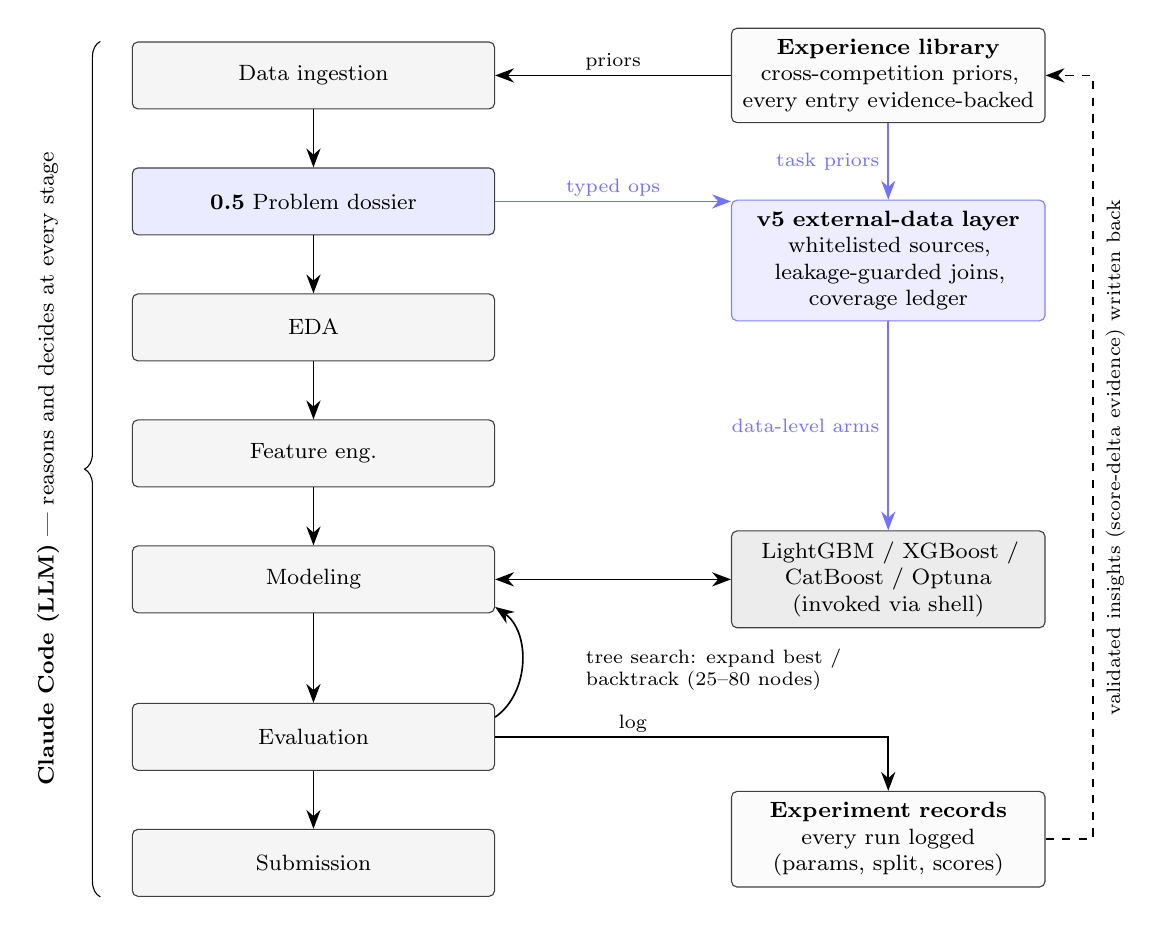
\begin{tikzpicture}[
  font=\footnotesize,
  stage/.style={draw=black!75, rounded corners=2pt, align=center, inner sep=3pt,
                fill=gray!8, minimum height=8.5mm, minimum width=46mm},
  supp/.style={draw=black!75, rounded corners=2pt, align=center, inner sep=4pt,
               fill=gray!3, text width=37mm},
  v5box/.style={supp, fill=blue!7, draw=blue!50},
  toolbox/.style={supp, fill=gray!15},
  arr/.style={-{Stealth[length=2.4mm]}, semithick},
  barr/.style={arr, blue!55},
  darr/.style={arr, dashed},
  lab/.style={font=\scriptsize, inner sep=1.5pt}
]
% ----- main pipeline (top -> bottom) -----
\node[stage]              (s1)  at (0,0)     {Data ingestion};
\node[stage, fill=blue!8] (s05) at (0,-1.6)  {\textbf{0.5} Problem dossier};
\node[stage]              (s2)  at (0,-3.2)  {EDA};
\node[stage]              (s3)  at (0,-4.8)  {Feature eng.};
\node[stage]              (s4)  at (0,-6.4)  {Modeling};
\node[stage]              (s5)  at (0,-8.4)  {Evaluation};
\node[stage]              (s6)  at (0,-10.0) {Submission};
\foreach \a/\b in {s1/s05, s05/s2, s2/s3, s3/s4, s4/s5, s5/s6}{\draw[arr] (\a) -- (\b);}
% ----- LLM annotation: vertical brace spanning all stages -----
\draw[decorate, decoration={brace, amplitude=2mm}]
  ([xshift=-4mm]s6.south west) -- ([xshift=-4mm]s1.north west)
  node[midway, xshift=-4mm, rotate=90, anchor=south]
  {\textbf{Claude Code (LLM)} --- reasons and decides at every stage};
% ----- tree-search loop (Evaluation -> Modeling), arc in the corridor -----
\draw[arr] ([yshift=2.5mm]s5.east) to[out=35, in=-35] ([yshift=-3.5mm]s4.east);
\node[lab, anchor=north west, align=left] at (3.4,-7.22)
  {tree search: expand best /\\backtrack (25--80 nodes)};
% ----- right rail -----
\node[supp]    (lib)   at (7.3,0)     {\textbf{Experience library}\\cross-competition priors, every entry evidence-backed};
\node[v5box]   (ext)   at (7.3,-2.35) {\textbf{v5 external-data layer}\\whitelisted sources,\\leakage-guarded joins,\\coverage ledger};
\node[toolbox] (tools) at (7.3,-6.4)  {LightGBM / XGBoost /\\CatBoost / Optuna\\(invoked via shell)};
\node[supp]    (rec)   at (7.3,-9.7)  {\textbf{Experiment records}\\every run logged (params, split, scores)};
% ----- rail / pipeline connections -----
\draw[arr]  (lib.west) -- node[lab, above]{priors} (s1.east);
\draw[barr] (lib.south) -- node[lab, anchor=east, xshift=-0.5mm]{task priors} (ext.north);
\draw[barr] (s05.east) -- node[lab, above]{typed ops} (ext.west |- s05.east);
\draw[barr] (ext.south) -- node[lab, anchor=east, xshift=-0.5mm]{data-level arms} (tools.north);
\draw[arr, {Stealth[length=2.4mm]}-{Stealth[length=2.4mm]}] (s4.east) -- (tools.west);
\draw[arr]  (s5.east) -- node[lab, above, pos=0.35]{log} (rec.north |- s5.east) -- (rec.north);
% ----- dashed write-back, up the far right -----
\draw[darr] (rec.east) -- ++(6mm,0) |- (lib.east);
\node[lab, rotate=90, anchor=north] at (10.0,-4.85)
  {validated insights (score-delta evidence) written back};
\end{tikzpicture}
\caption{Architecture of my-agent. The LLM drives every stage; modeling and evaluation iterate
via tree search, invoking Auto-ML tools through the shell, while the experience library and
experiment records close the evidence loop. Blue: the v5 injection layer
(Section~\ref{sec:v5}) --- the Stage 0.5 dossier emits typed operators that drive the
external-data layer, whose data-level arms race against the no-external baseline.}
\label{fig:arch}
\end{figure}

\paragraph{Tree-search protocol.} Every run in this report uses harness v3 (Figure~\ref{fig:tree}): ensembles are first-class node kinds with out-of-fold caching and weight search, and a budget phase machine exploits until all lineages plateau, then forces one exploration burst, then stops. A later v4 added external idea injection at the blend stage; no benchmark submission here used it (Section~\ref{sec:v5}).

\begin{figure}[htbp]
\centering
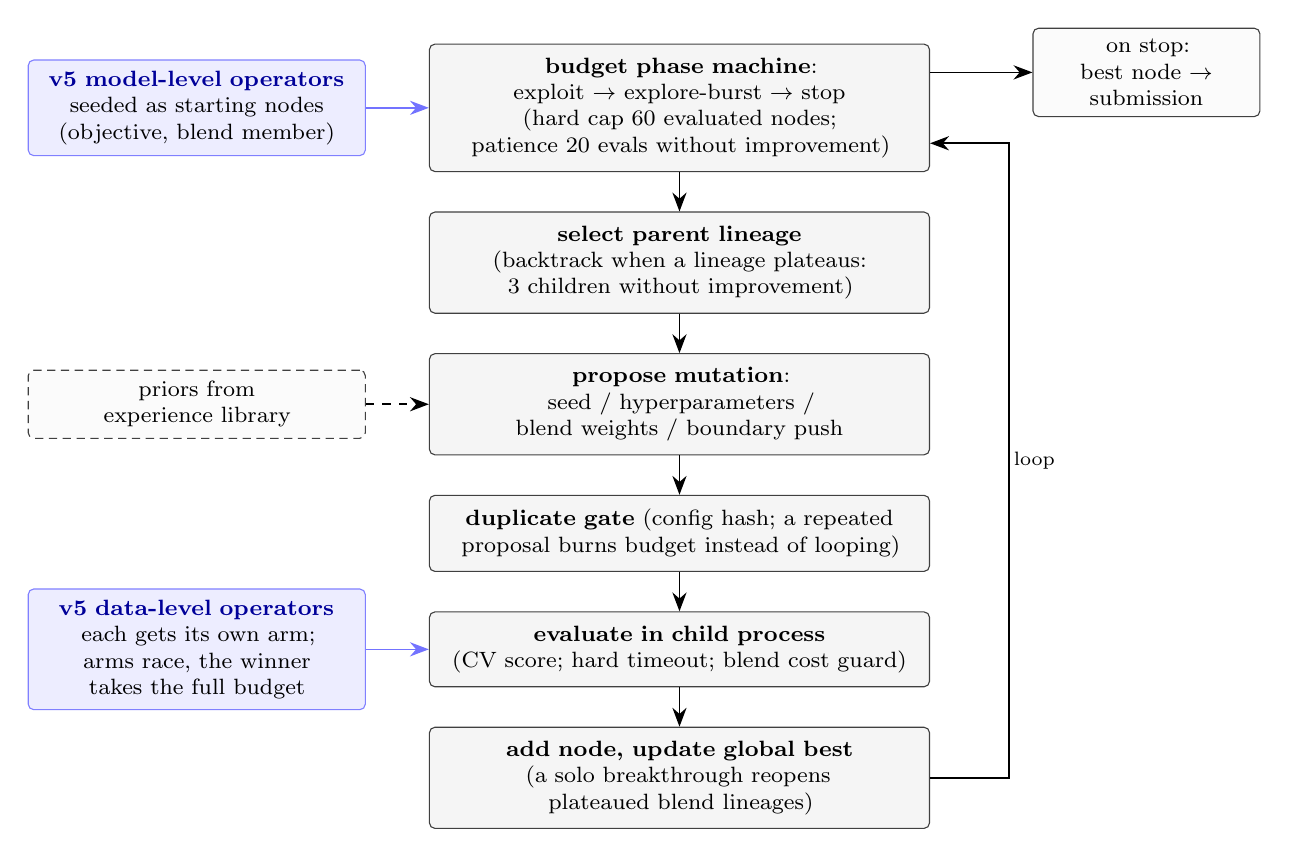
\begin{tikzpicture}[
  font=\footnotesize,
  sbox/.style={draw=black!75, rounded corners=2pt, align=center, inner sep=5pt,
               fill=gray!8, text width=60mm},
  sidebox/.style={draw=black!75, rounded corners=2pt, align=center, inner sep=4pt,
                  fill=gray!3, text width=40mm},
  v5side/.style={sidebox, fill=blue!7, draw=blue!50},
  arr/.style={-{Stealth[length=2.4mm]}, semithick},
  barr/.style={arr, blue!55},
  darr/.style={arr, dashed},
  lab/.style={font=\scriptsize, inner sep=1.5pt},
  node distance=5mm
]
% ----- main loop column -----
\node[sbox] (phase) {\textbf{budget phase machine}:\\exploit $\to$ explore-burst $\to$ stop\\(hard cap 60 evaluated nodes;\\patience 20 evals without improvement)};
\node[sbox, below=of phase] (select) {\textbf{select parent lineage}\\(backtrack when a lineage plateaus: 3 children without improvement)};
\node[sbox, below=of select] (propose) {\textbf{propose mutation}:\\seed / hyperparameters / blend weights / boundary push};
\node[sbox, below=of propose] (dedup) {\textbf{duplicate gate} (config hash; a repeated proposal burns budget instead of looping)};
\node[sbox, below=of dedup] (eval) {\textbf{evaluate in child process}\\(CV score; hard timeout; blend cost guard)};
\node[sbox, below=of eval] (add) {\textbf{add node, update global best}\\(a solo breakthrough reopens plateaued blend lineages)};
\foreach \a/\b in {phase/select, select/propose, propose/dedup, dedup/eval, eval/add}{\draw[arr] (\a) -- (\b);}
% ----- loop back, right side -----
\draw[arr] (add.east) -- ++(10mm,0) |- node[lab, pos=0.25, right]{loop} ([yshift=-4.5mm]phase.east);
% ----- exit, top right -----
\node[sidebox, text width=26mm, anchor=west] (out) at ([xshift=13mm, yshift=4.5mm]phase.east)
  {on stop:\\best node $\to$ submission};
\draw[arr] ([yshift=4.5mm]phase.east) -- (out.west);
% ----- side inputs, left column -----
\node[v5side, left=8mm of phase] (v5cfg)
  {\textcolor{blue!60!black}{\textbf{v5 model-level operators}}\\seeded as starting nodes\\(objective, blend member)};
\draw[barr] (v5cfg) -- (phase);
\node[sidebox, densely dashed, left=8mm of propose] (prior)
  {priors from\\experience library};
\draw[darr] (prior) -- (propose);
\node[v5side, left=8mm of eval] (v5data)
  {\textcolor{blue!60!black}{\textbf{v5 data-level operators}}\\each gets its own arm; arms race, the winner takes the full budget};
\draw[barr] (v5data) -- (eval);
\end{tikzpicture}
\caption{The v3 tree-search loop used in all my-agent runs of this report (22--80 nodes per
competition). Each node is a complete, executable solution scored by local cross-validation;
lineages are abandoned on plateau, and the budget phase machine forces one exploration burst
before stopping. Blue: v5's operator entry points (Section~\ref{sec:v5}) --- model-level
operators seed starting nodes; data-level operators build separately raced arms.}
\label{fig:tree}
\end{figure}

\subsection{The Injection Layer (v5): Dossier, External Data, and the Typed Contract}
\label{sec:v5}

The blue elements of Figures~\ref{fig:arch} and~\ref{fig:tree} form a single layer, and its placement carries the design argument. The v4 harness had injected external ideas downstream at the blend stage and measured a negligible effect (reweighting never displaced the convex-optimum champion in 8/8 rigorous competitions; pool expansion helped 2/8 by ${\sim}10^{-5}$); v5 moves the injection point upstream to problem identification, where the failure-mode analysis (Section~\ref{sec:exp4}) locates the shared gap of all three agents:

\paragraph{Stage 0.5 --- problem dossier.} Before EDA, the agent answers ``what kind of problem is this?'': task family, train--test window relation, split policy, and external-data need, written to a structured \path{dossier.json}. Judgments are grounded in \path{knowledge/task_priors.md}, a library of task-level priors each carrying an evidence field from our own benchmark (e.g., the shuffled-KFold $4.5\times$ bias; the GDP-join CV gap on jan-2022). Reading competition-specific discussions or kernels is forbidden --- the dossier must derive from the problem statement plus task-\emph{type} knowledge only, keeping the method distinct from reproduction-based agents. The dossier is a prior, not a conclusion: EDA must verify its hypotheses and record a verdict.

\paragraph{External-data module.} A whitelist of public sources (eleven World Bank indicators, ECB monthly FX, OWID COVID, holiday calendars, ISO tables), each fetched with recorded snapshots and joined through leakage-guarded as-of merges: an external value may reach a prediction row only if dated at or before the row's period minus a declared lag; violations raise an error; numeric time columns must declare their unit; every join writes an audit log. The module was adversarially verified (21 reproduced findings, including three silent-future-leak classes, all fixed with regression tests).

\paragraph{Search integration.} Data-level dossier ideas spawn their own variant workspaces raced at small tree-search budget; model-level ideas enter the main tree as seed lineages. The winning lane receives the full search budget.

\paragraph{A typed contract between the two layers.} The first version of this stack failed
instructively: the dossier correctly proposed World Bank GDP for s3e19 \emph{as a country-level
scale covariate}, and the experience library already held the operational recipe, but the
execution layer could express exactly one transformation --- appending a column to the feature
list. Since a gradient-boosted tree cannot extrapolate a feature beyond its training range, the
semantics of ``scale covariate'' evaporated between the layers with nothing raising an error.
The fix is a closed vocabulary both layers read (\path{knowledge/injection_operators.md}): ten
typed operators, each with a parameter schema, the evidence justifying it, and explicit
conditions under which it must \emph{not} be used. The dossier may emit only these, each
carrying its rationale and source prior; anything the vocabulary cannot express is written to
\texttt{not\_recorded} rather than into prose the execution layer will ignore. The dispatcher
writes a coverage ledger --- proposed, realized, unrealized-with-reason --- so an unimplemented
capability leaves a trace instead of resembling success. Two automatic preconditions guard the
level-covariate operators: proportionality and covariate volatility. Conformance is
machine-checked on both sides (Appendix~\ref{app:coverage}).

\subsection{Two Reference Methods (Yardsticks)}

\paragraph{AIDE} (open-source agent, gen-1): LLM-driven tree search. At each step it writes a complete solution, executes it, reads the error or score, and mutates accordingly. No cross-competition memory --- every competition starts from zero; the journal only persists within a single run.

\paragraph{NVIDIA Kaggle Agent} (skill): its method is ``reproduce the strongest public kernel'' --- research the competition context, select the highest-\emph{voted} solution-type kernel, port it faithfully, and retrain on local data.

\paragraph{Key methodological decision.} Both reference methods are frozen --- no improvements of any kind. During the study we found that NVIDIA's vote-based kernel selection is a structural weakness (Section~\ref{sec:exp4}), and the skill itself even ships a score-based selection tool, but we deliberately did not enable it. Rationale: the purpose of this study is to use them as fixed yardsticks for measuring my-agent; improving the yardsticks mid-study would make earlier and later data incomparable, and would quietly turn the benchmark into an optimization of the reference methods.

\section{Experimental Apparatus}
\label{sec:apparatus}

Two pieces of apparatus are prerequisites for every three-agent comparison and every
real-leaderboard verdict in this report, and neither is a finding in its own right: a fairness
protocol that makes a score attributable to a method rather than to an accident of the shared
machine, and an error model that says which score differences are readable at all. We state
both here, once, so that the experimental sections can report results without re-deriving the
conditions under which they mean anything. The offline-graded mid-complexity competitions of
Section~\ref{sec:exp7run2} are the one exception to the error model's reach, noted there.

\subsection{Fairness Protocol}
\label{sec:fairness}

The three agents share one machine, so four isolation conditions are defined and mechanically
enforced rather than left to convention (Table~\ref{tab:fairness}): if the agents could read each other's
files, or run concurrently on a contended machine, the win rates below would not be
attributable to method. Implementation details and the failure record are in the companion engineering log.

\begin{table}[htbp]
\centering\small
\caption{The four isolation conditions and what enforces each.}
\label{tab:fairness}
\begin{tabular}{@{}L{2.6cm}L{6.4cm}L{5.6cm}@{}}
\toprule
\textbf{Condition} & \textbf{Rule} & \textbf{Enforcement} \\
\midrule
Data & Each side reads only its own root, containing files validated against the official Kaggle manifest & \path{build_isolated_roots.py} \\
Workspace & The three output directories are fully separated; each side is scored independently & Directory structure \\
Instruction & Prompts may carry environment facts and metric thresholds only --- no modelling recipes, no other side's scores, no workaround discovered by another side & Manual protocol + incident log \\
Resource & Only one lane executes at any moment & \path{lane_lock.sh} mutex \\
\bottomrule
\end{tabular}
\end{table}

A fifth rule governs the experimenter rather than the agents: when the environment is
defective, fix the environment rather than hint to the affected side. Fixing removes the
confound; hinting compensates one side and silently changes what is being compared.

\subsection{The Paired Significance Test}
\label{sec:exp2}

\paragraph{Why an error model is needed at all.} Among the private-leaderboard results below (Table~\ref{tab:private}), several top-two gaps sit at the fourth or fifth decimal place (s5e10: 0.00003; s6e2: 0.00000). Do such gaps exceed measurement error? If not, the ``verdict'' is noise --- and a report that declares winners at that scale is reporting its own noise back to itself.

\paragraph{How --- the error scale comes from the data itself, not from assumptions.} Kaggle randomly splits each test set into two disjoint subsets, public and private, and one submission receives one score on each. These are two independent estimates of the same model, so their difference is that competition's metric sampling noise.

\paragraph{A failed first attempt, worth recording.} We initially used a single agent's own public--private gap as the threshold, and 8 of 10 competitions came out as ties. The reason is that this gap is mostly \emph{shared} across the three agents --- which rows land in which subset shifts everyone together. On s5e10 (Table~\ref{tab:drift}) the common shift is $0.00025$ against mutual scatter of only $0.00002$: using the common shift as the threshold inflates the true noise more than tenfold --- measuring a paired question with an unpaired scale.

\paragraph{The correct construction.} Measure how much the \emph{gap between two agents} moves across the two subsets --- the common drift cancels in the subtraction. Writing $d_{\mathrm{pub}}$ and $d_{\mathrm{priv}}$ for the between-agent score difference on the public and private subsets, a verdict requires both:
\begin{align}
\operatorname{sign}(d_{\mathrm{priv}}) &= \operatorname{sign}(d_{\mathrm{pub}})
  && \text{(the ordering replicates on disjoint samples)} \\
|d_{\mathrm{priv}}| &> |d_{\mathrm{priv}} - d_{\mathrm{pub}}|
  && \text{(the gap exceeds its own movement)}
\end{align}

\paragraph{Statistical properties of the decision rule.} Algebraically, condition~(2) is equivalent to $d_{\mathrm{pub}}\,(2d_{\mathrm{priv}} - d_{\mathrm{pub}}) > 0$ and therefore \emph{implies} condition~(1); we state both because they diagnose different failures. The rule is a conservative screen rather than a calibrated hypothesis test, but its false-verdict rate under a null model is computable. Suppose two agents are truly equivalent on a competition, so that $d_{\mathrm{pub}}$ and $d_{\mathrm{priv}}$ are independent zero-mean Gaussian noise with $\sigma_{\mathrm{pub}} = k\,\sigma_{\mathrm{priv}}$. The probability of a spurious verdict (in either direction) is
\begin{equation}
P_{\mathrm{FP}}(k) \;=\; \frac{1}{2} - \frac{\arctan(k/2)}{\pi},
\end{equation}
which gives $35.2\%$ for equal variances ($k=1$) and $25.0\%$ for the $20\%/80\%$ public/private splits common in these competitions (variance scales inversely with subset size, so $k \approx 2$); condition~(1) alone caps it at $50\%$ distribution-free.

\begin{table}[htbp]
\centering\small
\caption{Empirical evidence for common drift (excerpt). Drift = private minus public score of the same submission. In seven competitions the mutual scatter is less than half the common shift.}
\label{tab:drift}
\begin{tabular}{@{}lrrrrr@{}}
\toprule
\textbf{Competition} & \textbf{my-agent} & \textbf{NVIDIA} & \textbf{AIDE} & \textbf{Common shift} & \textbf{Mutual scatter} \\
\midrule
s5e10 & $+0.00025$ & $+0.00026$ & $+0.00024$ & $+0.00025$ & \textbf{0.00002} \\
s6e2  & $+0.00149$ & $+0.00160$ & $+0.00152$ & $+0.00154$ & 0.00011 \\
s3e11 & $+0.00063$ & $+0.00065$ & $+0.00056$ & $+0.00061$ & 0.00009 \\
s3e7  & $-0.00859$ & $-0.00772$ & $-0.00825$ & $-0.00819$ & 0.00087 \\
\bottomrule
\end{tabular}
\end{table}

\paragraph{Scope.} The test covers test-set sampling noise. The second error term --- between-run agent variance --- is measured separately for two of the three agents and reported with the results it affects (Sections~\ref{sec:limitations} and~\ref{sec:future}).

\section{The Three-Way Benchmark}

\subsection{Overview of Experimental Design}

\paragraph{Evaluation set.} 20 tabular competitions --- 14 from the Kaggle Playground Series, plus afsis-soil-properties (2014, spectral regression), conway-s-reverse-game-of-life (2014, structured multi-output), cat-in-the-dat (2019, purely categorical features), and tabular-playground aug-2022, jan-2022, and sep-2022. Every competition provides both a public and a private test-subset score --- the inclusion criterion required by the significance test (Section~\ref{sec:exp2}). The three agents also ran 4 competitions for which private scores cannot be obtained (late submission closed, rolling leaderboards); these are excluded. The study froze an 18-competition baseline; the two firing-class competitions (s5e1, tps-sep-2022) joined on 2026-07-31, when all three lanes ran them under benchmark conditions (Result 2c states the conditions, including my-agent's pinned knowledge library), bringing the baseline to 20.

\paragraph{Execution conditions.} The three agents ran serially under the mutex of Section~\ref{sec:fairness}. AIDE: 20 steps, its own default budget (conway stopped at 16 due to the 4-hour cap). NVIDIA: reproduced public kernels per its method. my-agent: the full six-stage pipeline including tree search (22--80 nodes per competition; Appendix~\ref{app:treesize}).

\subsection{Three-Way Capability Comparison (Raw Scores)}
\label{sec:exp1}

\paragraph{Goal and procedure.} Measure the absolute performance of the three methods on the same set of competitions. Each side independently produces a submission, uploaded to Kaggle via late submission to obtain public and private scores and a percentile rank (PR).

\begin{table}[htbp]
\centering\small
\caption{Competition descriptions. Tasks fall into two families: classification (binary, ordinal; 7 competitions) and prediction/regression (incl.\ time series and multi-target; 13 competitions).}
\label{tab:comps}
\begin{tabular}{@{}rllr@{}}
\toprule
\# & \textbf{Competition} & \textbf{Task type} & \textbf{Train rows $\times$ cols} \\
\midrule
1 & s3e1 & Regression & $37{,}137 \times 10$ \\
2 & s3e3 & Classification (binary) & $1{,}677 \times 35$ \\
3 & s3e5 & Classification (ordinal) & $2{,}056 \times 13$ \\
4 & s3e7 & Classification (binary) & $42{,}100 \times 19$ \\
5 & s3e9 & Regression & $5{,}407 \times 10$ \\
6 & s3e11 & Regression & $360{,}336 \times 17$ \\
7 & s3e14 & Regression & $15{,}289 \times 18$ \\
8 & s3e16 & Regression & $74{,}051 \times 10$ \\
9 & s3e19 & Regression (time series) & $136{,}950 \times 6$ \\
10 & s4e11 & Classification (binary) & $140{,}700 \times 20$ \\
11 & s5e10 & Regression & $517{,}754 \times 14$ \\
12 & s6e1 & Regression & $630{,}000 \times 13$ \\
13 & s6e2 & Classification (binary) & $630{,}000 \times 15$ \\
14 & afsis-soil-properties & Regression (multi-target) & $1{,}157 \times 3{,}600$ \\
15 & cat-in-the-dat & Classification (binary) & $300{,}000 \times 25$ \\
16 & conway-s-reverse-game-of-life & Structured multi-output & $50{,}000 \times 802$ \\
17 & tps-aug-2022 & Classification (binary) & $26{,}570 \times 26$ \\
18 & tps-jan-2022 & Regression (time series) & $26{,}298 \times 6$ \\
19 & s5e1 & Regression (time series) & $230{,}130 \times 6$ \\
20 & tps-sep-2022 & Regression (time series) & $70{,}128 \times 6$ \\
\bottomrule
\end{tabular}
\end{table}

\begin{table}[htbp]
\centering\small
\caption{Three-way performance, public leaderboard. \dn{} = lower is better, \up{} = higher is better; bold = best of the three scored columns. The \textbf{my-agent (v5)} column is the final-architecture Stage-0.5 re-run of Section~\ref{sec:rerun} --- its submissions exist but are unscored, so every cell is TBD; the \emph{pre-v5} column is the 2026-07 baseline runs, kept as the historical reference the analyses of this report were computed on.}
\label{tab:public}
\begin{tabular}{@{}rllcrrr@{}}
\toprule
\# & \textbf{Competition} & \textbf{Metric} & \textbf{my-agent (v5)} & \textbf{my-agent (pre-v5)} & \textbf{NVIDIA} & \textbf{AIDE} \\
\midrule
1 & s3e1 & RMSE \dn & TBD & 0.56083 & \textbf{0.55332} & 0.55899 \\
2 & s3e3 & ROC-AUC \up & TBD & 0.89262 & \textbf{0.93526} & 0.88484 \\
3 & s3e5 & QWK \up & TBD & 0.57921 & 0.57515 & \textbf{0.59362} \\
4 & s3e7 & ROC-AUC \up & TBD & 0.91116 & \textbf{0.91230} & 0.90934 \\
5 & s3e9 & RMSE \dn & TBD & 11.84951 & \textbf{11.83399} & 11.86657 \\
6 & s3e11 & RMSLE \dn & TBD & 0.29534 & 0.29559 & \textbf{0.29389} \\
7 & s3e14 & MAE \dn & TBD & 341.26711 & \textbf{338.36524} & 342.44918 \\
8 & s3e16 & MAE \dn & TBD & 1.34315 & \textbf{1.33566} & 1.33920 \\
9 & s3e19 & SMAPE \dn & TBD & 50.22497 & \textbf{47.52145} & 48.39715 \\
10 & s4e11 & Accuracy \up & TBD & 0.94125 & 0.94136 & \textbf{0.94184} \\
11 & s5e10 & RMSE \dn & TBD & \textbf{0.05551} & 0.05562 & 0.05555 \\
12 & s6e1 & Error \dn & TBD & \textbf{8.69338} & 8.70480 & 8.69449 \\
13 & s6e2 & ROC-AUC \up & TBD & \textbf{0.95367} & 0.95348 & 0.95364 \\
14 & afsis & MCRMSE \dn & TBD & \textbf{0.45207} & 0.61276 & 0.45636 \\
15 & cat-in-the-dat & ROC-AUC \up & TBD & \textbf{0.80801} & 0.77641 & 0.80790 \\
16 & conway & MAE \dn & TBD & \textbf{0.10771} & 0.11094 & 0.10960 \\
17 & tps-aug-2022 & ROC-AUC \up & TBD & \textbf{0.58559} & 0.57920 & 0.58479 \\
18 & tps-jan-2022 & SMAPE \dn & TBD & 4.90883 & \textbf{4.43958} & 10.11598 \\
19 & s5e1 & MAPE \dn & TBD & 0.10236 & \textbf{0.05726} & 0.12573 \\
20 & tps-sep-2022 & SMAPE \dn & TBD & 28.32738 & \textbf{4.77458} & 5.78998 \\
\bottomrule
\end{tabular}
\end{table}

\begin{table}[htbp]
\centering\footnotesize
\setlength{\tabcolsep}{3.5pt}
\caption{Three-way performance, private leaderboard; percentile rank (PR) in parentheses. In the verdict column, \M{} = my-agent, \N{} = NVIDIA, \A{} = AIDE; ``$>$'' means the gap passes the paired significance test of Section~\ref{sec:exp2}, ``$\approx$'' means indistinguishable within error. Bold = best of the three scored columns. The \textbf{my-agent (v5)} column is the Stage-0.5 final-architecture re-run (Section~\ref{sec:rerun}), unscored as of this draft (TBD); \emph{pre-v5} is the 2026-07 baseline runs, and the paired verdicts are computed on those historical lanes.}
\label{tab:private}
\begin{tabular}{@{}rllcrrrl@{}}
\toprule
\# & \textbf{Competition} & \textbf{Metric} & \textbf{my-agent (v5)} & \textbf{my-agent pre-v5 (PR)} & \textbf{NVIDIA (PR)} & \textbf{AIDE (PR)} & \textbf{Paired verdict} \\
\midrule
1 & s3e1 & RMSE \dn & TBD & 0.55987 (63.3) & \textbf{0.55550} (93.2) & 0.55552 (81.0) & $\N \approx \A > \M$ \\
2 & s3e3 & ROC-AUC \up & TBD & 0.87303 (29.4) & \textbf{0.89537} (66.8) & 0.86863 (26.4) & $\N > \M > \A$ \\
3 & s3e5 & QWK \up & TBD & \textbf{0.59743} (78.8) & 0.56974 (75.7) & 0.58138 (79.8) & $\M \approx \A > \N$ \\
4 & s3e7 & ROC-AUC \up & TBD & 0.90257 (74.3) & \textbf{0.90458} (78.1) & 0.90109 (67.1) & $\N > \M > \A$ \\
5 & s3e9 & RMSE \dn & TBD & 12.29871 (50.6) & \textbf{12.22913} (59.1) & 12.30667 (44.5) & $\N > \M \approx \A$ \\
6 & s3e11 & RMSLE \dn & TBD & 0.29597 (67.4) & 0.29624 (66.6) & \textbf{0.29445} (73.3) & $\A > \M > \N$ \\
7 & s3e14 & MAE \dn & TBD & 332.43560 (76.1) & \textbf{330.71616} (89.2) & 332.31556 (71.2) & $\N > \M$; other pairs $\approx$ \\
8 & s3e16 & MAE \dn & TBD & \textbf{1.33859} (84.2) & 1.34001 (96.4) & 1.34224 (91.4) & $\N > \A$; other pairs $\approx$ \\
9 & s3e19 & SMAPE \dn & TBD & 50.45537 (28.5) & \textbf{48.26558} (41.4) & 48.34131 (40.1) & $\N \approx \A > \M$ \\
10 & s4e11 & Accuracy \up & TBD & 0.94043 (50.7) & \textbf{0.94076} (52.8) & 0.94056 (62.1) & $\N > \M$; other pairs $\approx$ \\
11 & s5e10 & RMSE \dn & TBD & \textbf{0.05576} (85.7) & 0.05588 (59.4) & 0.05579 (78.9) & $\M > \A > \N$ \\
12 & s6e1 & Error \dn & TBD & \textbf{8.71733} (75.2) & 8.73239 (69.5) & 8.72191 (74.8) & $\M > \A > \N$ \\
13 & s6e2 & ROC-AUC \up & TBD & \textbf{0.95516} (78.8) & 0.95508 (63.0) & \textbf{0.95516} (76.5) & $\M \approx \A \approx \N$ \\
14 & afsis & MCRMSE \dn & TBD & \textbf{0.49517} (46.6) & 0.69855 (18.8) & 0.49861 (45.6) & $\M > \A > \N$ \\
15 & cat-in-the-dat & ROC-AUC \up & TBD & \textbf{0.80241} (73.1) & 0.77084 (32.6) & 0.80217 (70.3) & $\M > \A > \N$ \\
16 & conway & MAE \dn & TBD & \textbf{0.10875} (98.6) & 0.11189 (96.5) & 0.11065 (97.9) & $\M > \A > \N$ \\
17 & tps-aug-2022 & ROC-AUC \up & TBD & 0.59055 (66.0) & 0.58730 (43.0) & \textbf{0.59106} (60.5) & $\M \approx \A > \N$ \\
18 & tps-jan-2022 & SMAPE \dn & TBD & 6.46156 (71.5) & \textbf{4.63651} (76.4) & 10.66638 (28.9) & $\N > \M > \A$ \\
19 & s5e1 & MAPE \dn & TBD & \textbf{0.12752} (76.5) & 0.14594 (69.3) & 0.17917 (48.1) & $\M > \A$; other pairs $\approx$ \\
20 & tps-sep-2022 & SMAPE \dn & TBD & 28.54859 (14.6) & \textbf{5.48351} (80.3) & 9.72095 (48.3) & $\N > \A > \M$ \\
\midrule
\multicolumn{3}{@{}l}{Median PR (range)} & TBD & \textbf{72.3} (14.6--98.6) & 68.0 (18.8--96.5) & 68.7 (26.4--97.9) & \\
\bottomrule
\end{tabular}
\end{table}

PR is the share of that competition's final private standings the submission would beat (a would-be rank $r$ among $N$ teams gives $\mathrm{PR}=100\,(N-r)/N$, against the frozen final leaderboard) --- an \emph{absolute} capability reference (``where would this agent have placed had it entered?''), separate from the relative ordering among the three. On s3e19 the PRs of 28.5--41.4 show all three far behind typical participants; on s3e16 the PRs of 84.2--96.4 put all three in the top tier, where their small mutual gaps carry little practical meaning.

Public and private scores are shown in separate tables because the paired test (Section~\ref{sec:exp2}) is built on their difference. Under a naive ``bigger number wins'' count over the scored (pre-v5) columns, the tally is my-agent 8, NVIDIA 9, AIDE 2 (one M--A tie) --- a count the next section shows cannot be trusted. Per the study's version rule, the my-agent column of record for this benchmark is the Stage-0.5 final-architecture re-run; until its scoring step runs, every my-agent (v5) leaderboard cell is TBD, and all standings quoted in this report are those of the pre-v5 baseline lanes, labeled as such.

\subsection{Standing of the Three Agents Under the Paired Test}
\label{sec:winrates}

Applying the test of Section~\ref{sec:exp2} to all 60 duels of the \emph{pre-v5 baseline} lanes yields the standing below (the Stage-0.5 re-run re-enters this table once scored; Section~\ref{sec:rerun}). Against the rule's null false-verdict rate of roughly $25$--$35\%$, the observed decidable rate is $44/60 = 73\%$ --- far above what noise alone would produce, so most decided duels reflect genuine performance differences.

\begin{table}[htbp]
\centering\small
\caption{Paired-test results: 20 competitions $\times$ 3 pairings $= 60$ duels, of which 44 are decidable and 16 (27\%) are ties.}
\label{tab:winrates}
\begin{tabular}{@{}lrrr@{}}
\toprule
\textbf{Method} & \textbf{Wins} & \textbf{Losses} & \textbf{Win rate (excl.\ ties)} \\
\midrule
my-agent & 17 & 13 & \textbf{57\%} \\
NVIDIA   & 15 & 16 & 48\% \\
AIDE     & 12 & 15 & 44\% \\
\bottomrule
\end{tabular}
\end{table}

\paragraph{Interpretation.} my-agent leads (17/30 = 57\%; 95\% CI 37--76\% by competition-level cluster bootstrap, since duels within a competition are dependent); NVIDIA (48\%) and AIDE (44\%) are hard to separate within error, and over a quarter of all duels cannot be decided at all. The ranking is also sensitive to sample composition: restricted to the 14-competition Playground subset its winner flips (Section~\ref{sec:reversal}). Between-run agent variance, the second error term, revises several of these verdicts further (Section~\ref{sec:future}).

\section{Analysis: What the Benchmark Reveals}

The two studies in this section ran no new competitions: they are validated readings of the
benchmark's own artifacts --- its scores, logs, and champion code. They are separated from the
experiments because their evidence is observational, and they matter because each one changed
what we built next.

\subsection{Local CV and the Leaderboard Disagree}
\label{sec:exp3}

\paragraph{Why.} The attached per-competition specification reports (Appendix~\ref{app:specs}) compare the three agents on local CV, while the benchmark (Sections~\ref{sec:exp1} and~\ref{sec:winrates}) uses the actual leaderboard. If the two agree, CV is a reliable proxy and agent evaluation need not pay the cost of real submissions; if they disagree, every CV-based agent benchmark needs re-examination. The comparison is free --- both datasets already exist.

\paragraph{Result: 9 of 13 competitions disagree} (the comparison is limited to the 13 Playground competitions covered by the spec reports; CV verdicts, including their noise-floor tie calls, come from those reports' scored comparisons, and leaderboard verdicts from the paired test). The most extreme case, s3e19 (Table~\ref{tab:cvlb}), fully reverses direction: CV says my-agent leads by 3.7 points; the leaderboard says it trails by 2.2. Other disagreement patterns include: CV declares a tie while the LB separates the sides (s3e7, s3e9, s3e11, s5e10, s6e1), and CV declares a winner while the LB leaves that agent's duels undecided (s3e16).

\begin{table}[htbp]
\centering\small
\caption{The most extreme CV--LB disagreement, s3e19 (SMAPE, lower is better). CV numbers are a matched-split diagnostic pair (same TimeSeriesSplit for both agents), not the master table's champion CVs.}
\label{tab:cvlb}
\begin{tabular}{@{}lrrl@{}}
\toprule
\textbf{Basis} & \textbf{my-agent} & \textbf{NVIDIA} & \textbf{Verdict} \\
\midrule
Local CV (TimeSeriesSplit, same split for both) & 10.02 & 13.72 & my-agent by a wide margin \\
Private leaderboard & 50.46 & 48.27 & NVIDIA wins \\
\bottomrule
\end{tabular}
\end{table}

\paragraph{Why this happens.} CV and LB measure different things --- performance on resamples of the training data versus on a batch of never-seen data --- and they decouple as soon as the test--train relationship changes. s3e19 is the extreme case: the matched-split CVs sit at 10--14 (AIDE's own selected CV, 4.4, is the leaked shuffled-KFold number of Section~\ref{sec:exp4}) while the LB scores sit at 48--50, everyone misfiring together into the lower mode of a bimodal leaderboard (Section~\ref{sec:external}); the full mechanics are in the companion case-studies document.

\paragraph{Methodological implication.} Agent benchmarks must submit to the real leaderboard: CV is cheap and convenient, but its agreement rate here is only $4/13 = 31\%$ (95\% CI $9$--$61\%$). The attached per-competition reports are therefore explicitly labeled CV-only; their conclusions must not be mixed with the leaderboard verdicts of Table~\ref{tab:private}.

\subsection{Failure-Mode Analysis}
\label{sec:exp4}

Score tables cannot answer ``why.'' Reading the three agents' execution logs and champion code competition by competition reveals systematic method-level weaknesses --- worth more to agent design than any ranking.

\subsubsection{AIDE: Can Diagnose, but No Mechanism Lets the Diagnosis Veto the Score}

\paragraph{s3e16.} At steps 16 and 18 AIDE ran nested CV on its own initiative, measured calibrated values of 1.3396 / 1.3412, and wrote in its own report that ``the in-sample number is optimistic'' --- yet still selected the in-sample node. The private LB of 1.34224 confirms that the honest estimate it discarded was the correct one.

\paragraph{s3e19.} Worse. Mid-run, while fixing a LightGBM API issue, AIDE accidentally swapped its time-based validation for shuffled KFold. Its metric instantly ``improved'' from 18.42 to 4.41. The improvement was fake --- on time-series data, shuffling lets the model validate on rows from inside sequences it has already memorized --- but nothing flagged the jump, and AIDE spent its remaining nine steps tuning against the leaked number. A controlled experiment that changes only the split measures the illusion at $4.5\times$. my-agent ran the same shuffled split in the same competition, but tagged it ``diagnostic only'' and never submitted it. The full step trajectory and the controlled experiment are reconstructed in the companion case-studies document.

\subsubsection{NVIDIA: Votes Do Not Equal Quality}
\label{sec:votes}

The method selects kernels by votes, but votes measure popularity and pedagogical value. On s3e3, a battle-tested solution with only 89 votes (\path{chunweishen/ps-s03e03-ensembling}) took the three-way best, while high-vote kernels are often tutorial-oriented rather than competition-oriented (in a getting-started competition outside this report, a 7{,}859-vote tutorial kernel left NVIDIA last of the three). Moreover, the s3e19 kernel it reproduced (\path{tumpanjawat/s3e19-course-eda-fe-lightgbm}) claims in its header ``same idea as the 2nd-place solution''; NVIDIA faithfully reproduced its skeleton but missed the year-scaling step that decides the outcome (48.27 vs.\ the leaderboard top of 4.67) --- nothing in the method ever checks the reproduced score against the source's claimed rank.

\subsubsection{A Gap Shared by All Three: Recognizing the Need for External Data}
\label{sec:external}

The s3e19 leaderboard splits into two clusters with almost nobody in between: of 1{,}174 teams, 265 score below 10 while 570 land in 40--60 (percentile detail in the companion case-studies document). All three agents (private SMAPE 48.27, 48.34, 50.46) landed in the worse cluster. The teams in the better cluster did something none of the three agents did: they joined per-country GDP data.

\textbf{A correction we owe our own midterm.} The midterm blamed the missing GDP join for the whole gap. Measurement says otherwise. At matched budget the join is worth $-6.0$ SMAPE (Section~\ref{sec:exp6v5}), against a $\sim$44-point gap to the leader --- real, but small. The dominant obstacle is something else: the test set asks for a full future year of totals, an extrapolation that defeats every method in the comparison equally. There is a second lesson in how we got this wrong: our experience library already contained the correct diagnosis, but we retrieved and acted on a neighbouring entry that over-claimed. The library's weak link is retrieval, not content (Section~\ref{sec:future}; both entries are quoted in the companion case-studies document).

Even so, this is not a task-type ceiling: on the same-type tps-jan-2022, my-agent proactively joined World Bank GDP-per-capita data (CV SMAPE 4.1793), and AIDE, using only official data, discovered calendar and Black-Friday features on its own (6.1551).

\section{The Injection Layer: Controlled Experiments}

Acting on the diagnosis of Section~\ref{sec:exp4} --- problem-level judgment is the shared gap
of all three agents --- the experiments here evaluate the v5 layer of Section~\ref{sec:v5}
under the same leaderboard discipline as the benchmark: real submissions, judged by the paired
test of Section~\ref{sec:exp2}.

\subsection{Problem-Identification Sweep (Dossier Layer)}
\label{sec:exp5v5}

\paragraph{Design.} The dossier layer's generality claim is ``behaves correctly across the task distribution'': fire on tasks that genuinely need external data (sensitivity), stay silent on those that do not (specificity). We ran the dossier stage on all 18 original benchmark competitions --- LLM reasoning over the problem statement, data schema, and task priors only; minutes per competition; no training.

\paragraph{Result: perfect separation.} The layer fires on exactly the two country-panel time-series competitions --- s3e19 and jan-2022, the two whose accepted solutions are known to require external covariates --- and reports ``no / unlikely'' on all 16 iid-tabular, categorical, spectral, and structured-output competitions: sensitivity 2/2, specificity 16/16. (Two caveats keep this honest. The sensitivity half is partly in-sample: the task priors the dossier reads were distilled from this benchmark's own failure analysis of exactly these two competitions, so the 16/16 silence is the informative half, and 2/2 carries a 95\% CI reaching down to 16\%. And the two firing-class competitions added to the baseline later also fire, but they were \emph{selected} as firing-class, so the sweep claim rests on the original 18.) Two secondary behaviors: on s3e19 the dossier surfaced a genuine conflict --- a conservative setup-time \texttt{config.yaml} flag said external data was not allowed while the task prior's evidence implied otherwise --- and flagged it for verification rather than guessing (the official rules, Section 7.C, settle it in favor of permission); on the out-of-scope SIIM imaging competition it answers ``no'', correct within the current whitelist, whose source classes do not yet include prior-competition archives.

\subsection{What Upstream Injection Is Worth, and What Selects Its Form}
\label{sec:exp6v5}

\paragraph{Design.} s3e19 is the benchmark's canonical failure, so it is the causal test bed; tps-sep-2022 --- six-country daily sales, outside the frozen baseline, dossier written before any of the findings below --- is the held-out replication. For each competition we build arms whose processed feature tables are digit-identical to the baseline's plus whatever the operators add, so a configuration that drops the new columns reproduces the committed baseline score exactly (verified: difference 0.0). Each arm is submitted for real public and private scores and judged by the paired test of Section~\ref{sec:exp2}.

\paragraph{Result 1a: external-data injection works, robustly.} All four matched-budget comparisons beat the no-external baseline.

\begin{table}[H]
\centering\small
\caption{Matched-configuration arms: identical pipeline, no search, no blending, so the operator is the only difference. SMAPE, lower is better. Every external arm beats its own baseline and passes the paired test of Section~\ref{sec:exp2}. s5e1, which joined the firing class later, skipped this matched-configuration stage --- its pre-registered test ran searched arms only (Result 2b).}
\label{tab:v5-2x2}
\setlength{\tabcolsep}{5pt}
\begin{tabular}{@{}lrrrcrrrc@{}}
\toprule
 & \multicolumn{4}{c}{\textbf{s3e19}} & \multicolumn{4}{c}{\textbf{tps-sep-2022} (held out)} \\
\cmidrule(lr){2-5}\cmidrule(lr){6-9}
\textbf{Arm} & \textbf{CV} & \textbf{public} & \textbf{private} & \textbf{sig.} & \textbf{CV} & \textbf{public} & \textbf{private} & \textbf{sig.} \\
\midrule
no external data & 10.148 & 52.492 & 54.506 & --- & \textbf{11.348} & 23.828 & 25.476 & --- \\
\texttt{join\_feature} & 9.379 & \textbf{47.036} & \textbf{48.497} & yes & 11.624 & \textbf{21.973} & \textbf{23.390} & yes \\
\texttt{ratio\_target} & \textbf{7.793} & 50.853 & 52.073 & yes & 11.807 & 21.209 & 24.091 & yes \\
\bottomrule
\end{tabular}
\end{table}

Against the baseline: on s3e19 the feature join gains $6.01$ private SMAPE and the ratio target $2.43$; on sep-2022, $2.09$ and $1.39$. The paired movements are small relative to the gaps ($0.55$, $0.79$, $0.23$, $1.23$ respectively), so all four survive. The gated comparison against the frozen v3 baseline also passes with searched champions (v5 private 48.243 vs.\ v3 50.455; $d_{\mathrm{pub}}{+}3.389$, $d_{\mathrm{priv}}{+}2.212$, movement $1.177$), which lifts my-agent on s3e19 from clearly last (PR 28.5) to numerically first among the three agents.

\paragraph{Result 1b: the ordering survives a real search budget, and search does not rescue the weaker form.} At an equal 46-node budget per arm on tps-sep-2022, the no-external arm reaches CV $11.347$ / private $25.472$; \texttt{ratio\_target} $10.829$ / $23.774$; the gated variant (ratio paired with \texttt{sample\_weight} on 2020) $10.922$ / $23.973$. Both external arms beat the searched baseline and pass the paired test (movements $0.499$ and $0.577$ against gaps of $1.698$ and $1.499$). The informative comparison is across protocols: 46 nodes of search on the \emph{weaker} operator form ($23.774$) still lose to a \emph{single unsearched configuration} of the stronger one ($23.390$; a cross-protocol comparison, not a paired verdict) --- the choice of injection form is worth more than the entire search budget.

\paragraph{Result 2a: cross-validation cannot choose between the forms, and errs in opposite directions.} On s3e19 CV ranks \texttt{ratio\_target} best ($7.793$) while the leaderboard ranks it middle; on sep-2022 CV ranks \emph{both} external forms \emph{behind} the baseline while the leaderboard has both beating it significantly. A cross-validation whose folds all sit inside the training range cannot measure an operator whose purpose is extrapolation beyond it --- and on sep-2022 the last folds land on 2020, the year the proportionality diagnostic flags as broken (cross-country dispersion $0.466$ against ${\sim}0.01$ elsewhere), so the operator is scored twice on its worst case; we predicted the inversion from the fold boundaries before submitting. Nor is CV's verdict stable in the budget: at one node it ranks \texttt{ratio\_target} behind the baseline, at 46 nodes ahead; the leaderboard says ``ahead'' in both cases.

The diagnostic's own prescribed remedy --- down-weighting the broken 2020 to $0.3$ --- improves CV as designed ($11.807$ to $11.515$) but is slightly worse on the leaderboard (private $24.142$ vs.\ the ungated arm's $24.091$): CV misranks not only the operator choice but also the repair of a violated precondition. And a held-out-year protocol --- the obvious cheap substitute, whose validation geometry matches the task --- also fails: across three probes (s3e19 2021, sep-2022 2019 and 2020) it ranks \texttt{ratio\_target} first every time, while the leaderboard ranks \texttt{join\_feature} first on both competitions. Selecting the \emph{form} of an upstream injection is therefore not currently possible from local signals, and the leaderboard cannot stand in for them in a live competition.

\paragraph{Result 2b: a pre-registered selection rule, killed by its own test (s5e1).} After
the three probes above failed, one candidate selector remained standing: the proportionality
diagnostic, which had matched the outcome on both competitions --- but only in hindsight. A
fourth firing-class competition (playground-series-s5e1, ``Forecasting Sticker Sales''), which
the diagnostic read as the worst proportionality violation in the class, allowed a real test:
before any model was fitted or anything submitted, we committed a prediction to the
competition's dossier and to version control --- \texttt{ratio\_target} loses to
\texttt{join\_feature} here, by a larger relative margin than on either predecessor --- with
the falsifier stated alongside (the diagnostic's full reading of s5e1 and the panel-family
details are in the companion case-studies document).

The falsifier fired. Three 45-node searched arms, identical except for the operator's added
columns, scored public/private MAPE $0.14280/0.15751$ (baseline), $0.14193/0.15626$
(\texttt{join\_feature}), and $0.12057/\mathbf{0.12417}$ (\texttt{ratio\_target}) --- the predicted loser won by a 20\% relative
margin, paired-test significant on all three pairwise comparisons, with no remedy applied for
the violated years. Per the consequence pre-committed with the prediction, the proportionality
diagnostic is demoted from a gate to a recorded note: it describes the data honestly but does
not predict which operator form wins.

Three things follow. First, the injection claim itself \emph{replicates at $n{=}3$}: across
three competitions, all six external-data arms beat their no-external baselines, every one
paired-significant, s5e1 by the largest margin yet. Second, the form-selection problem hardens
rather than resolves: the form verdict is now split (\texttt{join\_feature},
\texttt{join\_feature}, \texttt{ratio\_target}), and every local signal tested is 0-for-3 ---
CV picked ratio/baseline/featurejoin where the leaderboard said featurejoin/featurejoin/ratio,
the held-out-year protocol misranked all three probes, and the proportionality diagnostic died on its first advance prediction. The operating rule is now: race both forms, always.
Third, the two 1-year-horizon competitions went to \texttt{join\_feature} and the one 3-year competition to \texttt{ratio\_target}, so horizon length may be the real selector --- but that is post-hoc pattern-matching, exactly the move the proportionality story was built on, and it earns belief only by pre-registration on the next firing competition. (jan-2022, the class's fourth member, is not a clean test bed --- its outcomes are already inside the prior library --- but its record, a ratio-family decomposition beating a GBDT at a 1-year horizon, is counter-evidence the horizon story will have to explain.)

\paragraph{Result 2c: the full three-way on the new firing-class competitions.} The
controlled arms above isolate operators; they do not say how the three \emph{agents} compare
on this class. Both new firing-class competitions were therefore run by all three agents
under benchmark conditions (these runs are what admitted s5e1 and sep-2022 into the 20-competition baseline of Section~\ref{sec:exp1}) --- my-agent's full pipeline with the knowledge library pinned,
for each lane, to the last commit before any information about that lane's own competition
entered it (its own leaderboard verdicts would be an answer key; class-level knowledge from
the sibling firing competitions, produced partly by this study's own leaderboard probes,
remained available --- an asymmetry the cold-start reference methods do not share); AIDE and NVIDIA frozen
exactly as in the main benchmark --- and every submission scored on the real leaderboard.

\begin{table}[H]
\centering\small
\caption{Firing-class three-way, real leaderboard (both metrics \dn). NVIDIA's public
scores match its source kernels' claimed LB digit-for-digit, verifying the faithful port.
Verdicts per the paired test of Section~\ref{sec:exp2}.}
\begin{tabular}{@{}llllll@{}}
\toprule
\textbf{Competition} & \textbf{Board} & \textbf{my-agent} & \textbf{NVIDIA} & \textbf{AIDE} & \textbf{Verdict} \\
\midrule
s5e1 (MAPE) & public & 0.10236 & \textbf{0.05726} & 0.12573 & \\
 & private & \textbf{0.12752} & 0.14594 & 0.17917 & $\M > \A$;\; \M{} vs \N{} sign-flip \\
\midrule
sep-2022 (SMAPE) & public & 28.32738 & \textbf{4.77458} & 5.78998 & \\
 & private & 28.54859 & \textbf{5.48351} & 9.72095 & $\N > \A > \M$ \\
\bottomrule
\end{tabular}
\end{table}

The private ranking reverses completely between two competitions of the same narrow class:
\M{}${>}$\N{}${>}$\A{} on s5e1, \N{}${>}$\A{}${>}$\M{} on sep-2022. Sharper still, on s5e1
the paired test refuses to order my-agent and NVIDIA at all: the public half of the test set
says NVIDIA by $0.045$, the private half says my-agent by $0.018$ --- the
evaluation-set caution of Section~\ref{sec:reversal}, that a ranking is a property of the
method \emph{and} the evaluation set, reproduced between the two disjoint halves of a single
competition's test split. The mechanism is
visible in the degradation: the vote-selected kernel was developed against the public board
it is tuned to ($0.057 \to 0.146$, $+155\%$, on s5e1), while my-agent's CV-driven pipeline
degrades least ($+24.6\%$) and takes the private board.

sep-2022 is the mirror image and NVIDIA's textbook win: a mature public solution exists (a
Ridge baseline, 277 votes), reproduction inherits it, and all three pairwise verdicts are
significant. my-agent's $28.5$ there is another CV--LB decoupling entry: its champion bet a
wrong 2021 regime from the pinned GDP prior with CV $4.67$; the lane's unchosen equal-share
arm scores $16.25$ private, submitted flagged as a diagnostic and not reported as an agent
result. One further observation closes the loop with the injection results: the s5e1 kernel
NVIDIA reproduced \emph{itself} joins external GDP-per-capita data --- the same covariate the
dossier layer identifies, both plausibly drawing on this competition family's shared folklore
--- so vote-selection
inherits the injection for free exactly when a mature public solution exists, and when the
public board misleads instead, the strategies separate.

\paragraph{Result 3: decomposing what remains, and correcting our own explanation.} Diagnostic probes --- global rescalings of the best arm, labelled as diagnostics and never reported as agent results --- separate level from shape on s3e19: roughly 15.5 points of the residual are a yearly-level error and roughly 33 remain as shape, against a leaderboard top of 4.67. The needed $1.6$ level multiplier is unlearnable in sample, external GDP data is worth $6.0$ of the 44-point gap --- the midterm correction recorded in Section~\ref{sec:external} --- and the experience library's other candidate recipe, multiplicative panel decomposition, fails to transfer here despite an apparently satisfied precondition. The probe grid, the in-sample evidence on the multiplier, and the full transfer test are in the companion case-studies document.

\paragraph{What the residual means for the report's central claim.} The same pipeline scores $11.59$ predicting 2021 from 2017--2020 and $48.497$ predicting 2022 from 2017--2021 --- a fourfold degradation from an identical procedure, which neither the level correction nor the structural recipe explains. That is Section~\ref{sec:exp3}'s ``everyone misfires together'' quantified: the final transition of a synthetic series can differ in kind from every transition inside the training window, and no in-sample protocol can anticipate it.

\paragraph{What the judgment layer proposes, and what actually consumes it.} Across the 20
dossiers the layer proposes 241 ideas. Counting those whose operator family exists gives 73\%;
tracing which are actually \emph{consumed} gives only 5\% at first measurement, because the three operators supplying most of
that headline were emitted into a key that no search driver read, while the dispatcher recorded them as
realized (now 27\%, after wiring a consumer and moving the target-free encodings into the data
layer). A produced artifact with no consumer is indistinguishable from a working one in every
log, score table and coverage metric --- and this instance occurred inside the very mechanism
built to prevent silent truncation. \textbf{An architecture claim needs a consumer trace, not a
vocabulary count.} Per-regime tables and audit scripts are in Appendix~\ref{app:coverage}.

\section{Generalization: Mid-Complexity Three-Way}
\label{sec:exp7run2}

\paragraph{Design.} The three agents re-run, each under its frozen method, on three competitions outside the tabular Playground family: us-patent-phrase-to-phrase-matching (NLP, text pairing), ventilator-pressure-prediction (physiological time series), and SIIM-ISIC melanoma (dermoscopic imaging) --- machine fully dedicated per lane, 4--8h budgets, same isolation protocol. This tests whether the Playground conclusions (ranking reversal, CV--LB decoupling, failure modes) extend beyond the task family they were measured on. Version discipline: none of the three lanes ran the v5 injection layer (per-lane detail in Section~\ref{sec:limitations}). Search discipline: none of the three lanes used tree search --- a node here is a full deep-learning fine-tune (30--90 minutes, versus seconds for a tabular GBDT refit), so the prescribed 25--80 node budget would cost 15--100+ GPU-hours against the 4--8h available. All three took the skill's documented fallback for exactly this condition: one linear pass to a validated single model plus a blend, with the high-leverage moves (backbone choice, seed bagging, blend weights) taken directly.

\paragraph{Scoring.} The mid-complexity competitions use MLE-bench~\cite{mlebench} prepared splits and are graded offline against the held-out private split (us-patent is a code competition and ventilator/SIIM live test sets differ from the prepared splits, so Kaggle late submission is structurally unavailable); medal thresholds and the above-median flag come from the frozen leaderboard snapshot.

\paragraph{Results.}
\begin{table}[H]
\centering\small
\caption{Mid-complexity three-way, offline-graded against the held-out private split. Bold = three-way best; $\dagger$ = above the frozen leaderboard's median.}
\begin{tabular}{@{}lllll@{}}
\toprule
\textbf{Competition} & \textbf{Metric} & \textbf{my-agent} & \textbf{NVIDIA} & \textbf{AIDE} \\
\midrule
us-patent & Pearson $r$ \up & \textbf{0.86658}$\dagger$ (silver) & 0.86160$\dagger$ (bronze) & 0.65821 \\
ventilator & MAE \dn & \textbf{0.16525} & 0.40093 & 0.34591 \\
SIIM-ISIC & AUC \up & \textbf{0.93529}$\dagger$ & 0.89822 & 0.88579 \\
\bottomrule
\end{tabular}
\end{table}

my-agent takes the three-way best on all three and the only above-median score on SIIM --- a cleaner sweep than on the Playground set, where its edge was narrow and evaluation-set dependent. The three task families are unrelated, so the result is about pipeline discipline rather than tabular-specific tuning. Offline grading yields one score per submission, so the paired public/private test of Section~\ref{sec:exp2} does not apply here.

\section{The Final-Architecture Re-Run (In Progress)}
\label{sec:rerun}

\paragraph{Why a re-run.} The 20 my-agent lanes of Section~\ref{sec:exp1} were produced across the study's own development timeline, so different competitions ran different architecture vintages --- by the end of the study s3e1's workspace held 13 candidate evaluators and s5e1's held 7, and ``re-run with the final architecture'' would have meant a different thing on every relaunch (2026-08-04 finding). A re-run manifest (\path{docs/rerun_manifest.json}) now fixes exactly one workspace, one canonical evaluator and one search driver per competition, and all 20 competitions re-run under that frozen definition. The reference lanes do not move: AIDE and NVIDIA stay the frozen yardstick columns of Table~\ref{tab:private}, and the re-run will be placed against them by the same paired test once scored.

\paragraph{Enforcement, tightened beyond Section~\ref{sec:fairness}.} Each lane runs in an isolated root whose data files are validated against the official Kaggle manifest, holds \emph{no credentials} (the Kaggle token is stripped from the environment; a lane can neither consult the leaderboard nor submit), sees only its own workspace (the other nineteen are unreadable), and is denied the answer-key and out-of-fold cache channels that an earlier audit found reachable. New in this run: a \emph{per-lane transcript audit} reads every tool call the lane made --- detectors for network access, raw opens of the shared knowledge library that bypass the query interface's self-citation exclusion, and results of sibling benchmark competitions appearing without a sanctioned source --- and the launcher halts the whole queue after two consecutive audit failures, on the reasoning that two in a row indicts the pipeline rather than one lane.

\paragraph{Timeline.} The queue launched 2026-08-14 10:43 after operator approval and ran 14 lanes (13 of them writing submissions) by 08-15 02:05, when it aborted at a lane boundary: the Kaggle OAuth token had been revoked (HTTP 401) and the launcher reads a sub-minute lane exit as an environment fault, not a result. It resumed 08-17 after token triage, re-ran the three lanes that needed it (below), halted once more on the two-consecutive-audit-failures rule, and resumed again at 15:26 with s6e1 --- in flight as this draft compiles.

\paragraph{The audit gate, exercised in both directions.} Three incidents, each resolved by reading the transcript rather than trusting either the lane or the auditor:
\begin{itemize}[leftmargin=*]
  \item \textbf{s3e19, first attempt discarded --- real contamination.} The 08-14 lane opened the raw knowledge library four times and issued a genuine socket-opening command; the audit blocked it. The clean 08-17 re-run scores \emph{worse} on local CV (pooled OOF SMAPE 6.706 against the tainted attempt's 5.740) --- consistent with the contamination advantage being real, and with the audit pricing it correctly.
  \item \textbf{s3e19, re-run flagged --- auditor false positive.} The network detector matches the substring \texttt{kaggle} anywhere in a command, and fired on an \texttt{ls} of a directory named \path{kaggle-safe-submit}. A manual scan of all 118 tool calls in the re-run transcript found zero network commands; the result was accepted under a recorded operator waiver, and the detector fix is queued for after the run (the run root is baseline-frozen, so mid-run edits would invalidate the remaining lanes).
  \item \textbf{s5e10 --- score untainted, write-back in violation.} The audit flagged four raw library opens. The transcript timeline places every one of them strictly \emph{after} the submission was written and validated (tool-call indices 318--337 versus 302--306), with all modeling-phase library access going through the sanctioned query interface --- so the score stands. The genuine violation was different: the lane hand-edited the \emph{shared} knowledge library after finalisation, the channel by which one lane's outcomes could poison later lanes' priors. The library was surgically reverted, and no later lane consumed the polluted version because the queue had already halted before s6e1 started.
\end{itemize}

\paragraph{Progress and local numbers.} 15 of 20 lanes are complete (${\sim}17$ hours of lane time), one is running, four are queued. Because lanes hold no credentials, \emph{nothing in this section has touched the leaderboard yet}: scoring is a separate operator step, and every leaderboard cell below is TBD until it runs. The local numbers are each lane's own honest out-of-fold estimate (leave-fold-out where the lane measured its weight-fitting optimism), quoted for progress only --- Section~\ref{sec:exp3} showed local CV contradicting the leaderboard in 9 of 13 competitions, and this table re-illustrates the point (s3e19's pooled OOF SMAPE of 6.71 sits against baseline leaderboard SMAPEs near 50), so no comparative claim is made from them.

\begin{table}[H]
\centering\footnotesize
\setlength{\tabcolsep}{4pt}
\caption{Final-architecture re-run: state as of 2026-08-17 (evening). Local CV = the lane's honest OOF estimate, not leaderboard-validated; public/private leaderboard scores for all lanes are TBD pending the operator scoring step.}
\label{tab:rerunprog}
\begin{tabular}{@{}rllrrl@{}}
\toprule
\# & \textbf{Competition} & \textbf{Metric} & \textbf{Local CV (OOF)} & \textbf{Minutes} & \textbf{Lane status} \\
\midrule
1 & s3e1 & RMSE \dn & 0.548862 & 30 & done 08-14 \\
2 & s3e3 & ROC-AUC \up & 0.841605 & 20 & done 08-14 \\
3 & s3e5 & QWK \up & 0.571980 & 46 & done 08-14 \\
4 & s3e7 & ROC-AUC \up & 0.901769 & 50 & done 08-14 \\
5 & s3e9 & RMSE \dn & 12.082282 & 28 & done 08-14 \\
6 & s3e11 & RMSLE \dn & 0.292886 & 107 & done 08-17 (first attempt exited without a submission) \\
7 & s3e14 & MAE \dn & 340.95936 & 27 & done 08-14 \\
8 & s3e16 & MAE \dn & 1.334958 & 45 & done 08-14 \\
9 & s3e19 & SMAPE \dn & 6.70585 & 39 & done 08-17 (clean re-run; first attempt discarded by audit) \\
10 & s4e11 & Accuracy \up & 0.940810 & 81 & done 08-14 \\
11 & s5e10 & RMSE \dn & 0.055971 & 72 & done 08-17 (audit incident resolved, score accepted) \\
12 & s6e1 & Error \dn & TBD & --- & \textbf{running} (started 08-17 15:26) \\
13 & s6e2 & ROC-AUC \up & TBD & --- & queued \\
14 & afsis & MCRMSE \dn & 0.470503 & 24 & done 08-14 \\
15 & cat-in-the-dat & ROC-AUC \up & 0.803272 & 140 & done 08-14 \\
16 & conway & MAE \dn & 0.106688 & 214 & done 08-14 \\
17 & tps-aug-2022 & ROC-AUC \up & TBD & --- & queued \\
18 & tps-jan-2022 & SMAPE \dn & TBD & --- & queued \\
19 & s5e1 & MAPE \dn & 5.84\% & 113 & done 08-15 (cross-arm weights in-sample; see note) \\
20 & tps-sep-2022 & SMAPE \dn & TBD & --- & queued \\
\midrule
\multicolumn{6}{@{}l}{\emph{Leaderboard scoring (all 20 lanes): \textbf{TBD} --- runs as a separate credentialed operator step after the last lane.}} \\
\bottomrule
\end{tabular}
\end{table}

\noindent\emph{Note on s5e1:} the lane's cross-arm blend weights and global scale are fitted on the same OOF rows they are scored on, so its 5.84\% is optimistic relative to a held-out estimate --- the lane's own summary records this caveat.

\paragraph{What happens next.} After the last lane, the operator scoring step submits each lane's frozen \path{submission.csv} for real public/private scores (\path{score_lane_submissions.py}; dry-run by default, real submission behind an explicit flag), and \path{build_rerun_three_way.py} places the re-run column next to the frozen AIDE/NVIDIA yardsticks under the paired test of Section~\ref{sec:exp2}. Until then, every standing reported elsewhere in this document is the baseline's; nothing in this section revises any of it.

\section{Discussion}

\subsection{Contributions}

\begin{enumerate}[leftmargin=*]
  \item \textbf{An end-to-end competition agent whose knowledge enters at problem
  identification rather than at blending} --- with the limits of that claim stated. The agent
  runs the full pipeline under LLM control with Auto-ML tools, an experience library, and a
  tree-search optimisation loop; the architectural change this report argues for is the
  upstream dossier layer. It separates cleanly on the benchmark (fires on exactly 2 of 18, no
  false positives), and in matched-configuration designs every external-data arm beats its own
  baseline significantly --- six of six across three firing-class competitions --- against the
  near-null effect the same pipeline measured at the blend stage (different competitions and
  metric scales; the contrast is qualitative, not a same-unit ratio). What we
  cannot do is choose which \emph{form} the injection should take: every local signal tested is
  0-for-3, including a diagnostic we believed enough to pre-register a prediction on --- which
  its own named falsifier then killed.

  \item \textbf{The agent's standing against two frozen, methodologically distinct yardsticks.}
  57\% of decidable duels across 20 tabular competitions, the three-way best on all three
  mid-complexity competitions (NLP, physiological time series, medical imaging), and a
  characterisation of \emph{where} the advantage lives: concentrated where no mature public
  solution exists, absent where one does (Section~\ref{sec:votes}).

  \item \textbf{Two cautions that constrain how any such claim may be stated.} A ranking is a
  property of method $\times$ evaluation set --- same agents, same test, two reasonable
  competition sets, and the winner flips (Section~\ref{sec:reversal}) --- and local
  cross-validation is not a proxy for the leaderboard, disagreeing in 9 of 13 competitions and
  fully reversing direction on s3e19 (Section~\ref{sec:exp3}). Both are demonstrated rather
  than asserted, and both apply to our own agent first.

  \item \textbf{Measurement apparatus, offered for reuse.} A paired significance test that
  costs no extra experiments --- Kaggle's own public/private split supplies the error scale
  (Section~\ref{sec:exp2}) --- together with a direct measurement of between-run agent variance
  (Section~\ref{sec:future}). Applied here they find 27\% of duels undecidable before variance
  is even counted, and revise further verdicts once it is. This is infrastructure rather than a
  finding, but without it none of the numbers above would be readable.
\end{enumerate}

\subsection{Comparing the Three Methods}

The differences lie not in tuning skill but in where knowledge comes from and how the next step is decided (Table~\ref{tab:threeway}).

\begin{table}[htbp]
\centering\footnotesize
\setlength{\tabcolsep}{4pt}
\caption{Design comparison of the three methods.}
\label{tab:threeway}
\begin{tabular}{@{}L{3.2cm}L{4.2cm}L{3.4cm}L{3.6cm}@{}}
\toprule
\textbf{Aspect} & \textbf{my-agent} & \textbf{AIDE} & \textbf{NVIDIA} \\
\midrule
Knowledge source & Cross-competition experience library (accumulating) & None (from zero each time) & Public kernels fetched fresh each time \\
Search strategy & Six-stage pipeline + tree search (25--80 nodes) & Tree-shaped trial and error, 20 steps & No search; faithful reproduction \\
Basis for next step & Experience-library priors + OOF diagnostics & Previous step's error or score & Highest-voted kernel \\
Validation rigor & Split chosen by task type; diagnostics tagged and excluded & No concept of split legality & Inherits the kernel's split \\
External data & Proactively joined (GDP in jan-2022) & Never considered & Inherited from the kernel \\
Paired win rate (20 comps) & \textbf{57\%} & 44\% & 48\% \\
\bottomrule
\end{tabular}
\end{table}

\paragraph{Respective strengths.}
\begin{itemize}[leftmargin=*]
\item \textbf{NVIDIA's strength is standing on shoulders, not its own reasoning.} It wins on s3e3, s3e7, s3e9, s3e14, and jan-2022 --- competitions with mature, high-quality public solutions. It skips the entire exploration process and directly harvests hundreds of community person-hours, which is highly efficient whenever a good public solution exists; within the 14-competition Playground subset its win rate is actually the highest of the three (58\%).
\item \textbf{AIDE's strength is search depth.} s3e11 is its only outright first place, and the edge came from a bug-fix node that accidentally enabled native categorical handling --- massive trial and error stumbles into combinations a person would not think of. It needs no external knowledge to operate.
\item \textbf{my-agent's strength is validation rigor and knowledge accumulation.} It takes outright first on s5e10 and s6e1, and places high on s3e5 and s3e16. More important is the methodological layer: facing the same shuffled-KFold trap on s3e19 (Section~\ref{sec:exp4}), AIDE misused it for its official submission while my-agent quarantined it --- a distinction that never shows up in a single score, yet determines reliability on unseen tasks.
\end{itemize}

\paragraph{Respective limitations.}
\begin{itemize}[leftmargin=*]
\item \textbf{NVIDIA's bottleneck is its selection signal.} Votes measure popularity, not quality (Section~\ref{sec:votes}); it never checks the reproduced score against the source's claimed rank, and when no public solution exists, the method has nothing to work with --- and its one-shot execution is all-or-nothing: when process discipline lapses, there is no fallback, where iterative search always holds a submittable solution (engineering log, ventilator reconstruction).
\item \textbf{AIDE's bottleneck is the missing mechanism to let diagnoses veto scores.} It can produce correct diagnoses yet still choose the optimistic node (s3e16), and on s3e19 its own metric improved $4\times$ in one step without raising any alarm (Section~\ref{sec:exp4}). It optimizes the displayed number, not true performance.
\item \textbf{my-agent's bottleneck is judgment at the problem-identification level.} The experience library holds validated techniques (``use an L1 objective for MAE tasks''), but s3e19 required the upstream judgment ``this task needs external data,'' where the library has no leverage --- and on jan-2022, my-agent joined GDP data yet still lost to the kernel NVIDIA reproduced, showing a gap between having the right idea and executing it fully. Moreover, its 57\% lead is concentrated in the 6 non-Playground competitions; within the Playground subset it sits at 47\% (Section~\ref{sec:reversal}).
\end{itemize}

\paragraph{Shared limitation.} On s3e19 all three landed in the lower mode of the bimodal leaderboard, none recognizing the need for GDP data --- a per-competition miss, not a task-type ceiling (Section~\ref{sec:external}). Section~\ref{sec:exp6v5} sharpens this: the join is worth $6.0$ SMAPE, but the shared shortfall is mostly a one-year extrapolation no method in the comparison addresses.

\subsection{A Ranking Is Not a Property of the Method, but of Method $\times$ Evaluation Set}
\label{sec:reversal}

The most important methodological lesson of this study: same agents, same test --- swap the competition set and the ranking fully reverses (Table~\ref{tab:reversal}).

\begin{table}[htbp]
\centering\small
\caption{Ranking reversal across evaluation sets.}
\label{tab:reversal}
\begin{tabular}{@{}lrrr@{}}
\toprule
\textbf{Evaluation set} & \textbf{my-agent} & \textbf{AIDE} & \textbf{NVIDIA} \\
\midrule
Playground subset, 14 comps (win rate) & 47\% & 44\% (last) & \textbf{58\%} (first) \\
Full baseline, 20 comps (win rate) & \textbf{57\%} (first) & 44\% (last) & 48\% \\
Median PR (14 comps) & \textbf{74.8} & 72.2 & 68.0 \\
Median PR (20 comps) & \textbf{72.3} & 68.7 & 68.0 \\
\bottomrule
\end{tabular}
\end{table}

The reversal mechanism is clearly identifiable and maps directly onto each method's knowledge source. Three of the six non-Playground competitions are old or non-mainstream (afsis 2014, conway 2014, cat-in-the-dat 2019): their public kernels are either stale or tutorial-grade, so NVIDIA's ``reproduce the top-voted kernel'' loses the mature solution ecosystem it enjoys in the Playground series --- its PR drops to 18.8 (afsis) and 32.6 (cat-in-the-dat). Across the six non-Playground competitions my-agent goes 8W--3L while NVIDIA goes 4W--8L --- not because my-agent got stronger, but because its opponent's precondition disappeared. The exception proves the mechanism: sep-2022, the one non-Playground competition with a mature public solution (a 277-vote Ridge baseline), is NVIDIA's cleanest win in the set.

Two observations:

\begin{enumerate}[leftmargin=*]
  \item \textbf{Median PR orders the three identically on both evaluation sets} (my-agent $>$ AIDE $>$ NVIDIA), while the paired win rate reverses. Absolute-position metrics are more stable than relative verdicts, because the latter binarize many near-tie gaps and are therefore highly sensitive to sample composition.
  \item \textbf{``Which agent is stronger'' is an incomplete question.} The correct question is ``stronger on what distribution of competitions'': with mature public solutions, reproduction (NVIDIA) dominates; on obscure, old, build-your-own-pipeline tasks, autonomous methods (my-agent) dominate. Any single-number benchmark ranking hides an unstated assumption about the competition distribution.
\end{enumerate}

\paragraph{Methodological implication.} An agent benchmark's conclusion must be stated together with the composition of its evaluation set, and should report both an absolute metric (PR) and a relative one (paired win rate).

\subsection{Limitations of the Experimental Design}
\label{sec:limitations}

\begin{itemize}[leftmargin=*]
  \item \textbf{The significance test covers only test-set sampling noise}, not between-run agent variance. That variance is now measured for my-agent and AIDE on four competitions (Section~\ref{sec:future}) --- and where measured, it does revert several fourth-decimal verdicts to ties; NVIDIA's term remains unmeasured.
  \item \textbf{The duels are not independent trials.} Each competition contributes three
  duels that are deterministic functions of six shared scores, and each submission enters two
  duels, so duel-iid intervals are anti-conservative and the effective sample size is closer to 20
  competitions than to 30 duels (five competitions produce the identical full sweep
  $\M > \A > \N$, making the correlation visible). The intervals quoted in this report are
  therefore competition-level cluster bootstrap (20{,}000 resamples): my-agent 57\% [37, 76],
  NVIDIA 48\% [25, 73], AIDE 44\% [28, 62] --- materially wider for NVIDIA than the naive
  intervals. A further asymmetry touches every NVIDIA duel: reproduced kernels were tuned by
  their authors against the realized public leaderboard, so NVIDIA's public score is not an
  unbiased estimate of its private one. Across the 20 competitions the median public-to-private
  degradation is small for all three ($+0.5$ to $+0.8\%$), but NVIDIA's distribution sits
  highest --- IQR $[+0.3, +3.6]\%$ against my-agent's $[-0.2, +1.3]\%$ --- and holds the
  extreme ($+155\%$, s5e1). The paired test's exchangeability premise is weakest exactly where
  the reproduction method is strongest.
  \item \textbf{Budgets are per-method conventions, not compute-matched.} AIDE runs its
  default 20 steps, my-agent 22--80 evaluated nodes plus a linear pass, NVIDIA minutes of
  reproduction; each method runs ``as shipped,'' so the win rates compare methods-with-their-budgets,
  not methods at equal compute.
  \item \textbf{The baseline expansion was post hoc.} The two firing-class competitions'
  leaderboards had been consulted for the injection experiments before their three-way lanes
  ran; under the frozen 18-competition set the rates were 59\% (M), 45\% (N), 46\% (A).
  Both sets are reported so the reader can see exactly what the addition moved (it swapped
  second place).
  \item \textbf{The asymmetry created by the experience library is disclosed, not eliminated.} my-agent carries cross-competition memory; the other two cold-start --- a design difference rather than a flaw, but it colors the interpretation of the conclusions.
  \item \textbf{The sample is small, and Section~\ref{sec:reversal} shows the ranking is sensitive to set composition.} With 20 competitions and 60 duels, the gap between 57\% and 44\% remains a rough estimate; adding or removing a single competition can move it by one to two percentage points --- the two firing-class additions themselves moved every rate and swapped second place. The bootstrap intervals of the preceding bullet make this concrete --- all three overlap substantially.
\end{itemize}

\subsection{Open Problems}
\label{sec:future}

Four questions this study leaves open, ordered by how much they would change its conclusions.

\paragraph{Between-run agent variance --- now measured for two of the three agents.} On the
four competitions with the benchmark's tightest duels, my-agent ran twice fresh under
identical current conditions (fresh workspace, knowledge library pinned per competition to
the last commit before any information about that competition entered it; two runs rather
than one because the original baselines executed at older skill commits, so a fresh-vs-baseline
gap would confound run noise with version drift), and AIDE's pinned re-run pairs against its
frozen baseline. Private-leaderboard spreads:

\begin{center}\small
\begin{tabular}{@{}lccc@{}}
\toprule
 & \textbf{my-agent} & \textbf{AIDE} & \textbf{baseline duel gaps} \\
\midrule
s4e11 & 0.00021 & 0.00027 & 0.00013--0.00033 \\
s3e16 & 0.00460 & 0.00056 & 0.00142--0.00365 \\
s5e10 & 0.00000 & 0.00003 & 0.00003--0.00012 \\
s6e2  & 0.00000 & 0.00020 & 0.00000--0.00008 \\
\bottomrule
\end{tabular}
\end{center}

Three readings. First, the consequence the limitation predicted is real: of the twelve
pairwise duels on these four competitions, eight are undecidable under the combined error
model --- seven at gaps at or below a measured wobble (including s5e10's M${>}$A, previously
a significant win, whose $0.00003$ gap exactly equals AIDE's wobble there), one by the
paired sampling test alone; the four that survive all involve NVIDIA, the one agent whose
variance remains unmeasured. Second, the variance is substantially a property of the
\emph{task}, not the agent: both agents agree s3e16 is the noisy competition by an order of
magnitude, so error bars must be per-competition, not one global number. Third, the
pipeline's endpoint is far more stable than its route --- my-agent's two runs took visibly
different paths on every competition (a linear-protocol blend versus a 60-node tree search
on s4e11; a top-30 equal blend versus a 19-node greedy selection on s3e16) yet landed
within $0.0002$ everywhere except the task both agents find noisy. What remains open:
NVIDIA's variance term, and widening the sample beyond the four comps measured.

\paragraph{Operator form cannot be selected from any local signal we have tested --- now
0-for-3, with one selector killed by pre-registration.} Section~\ref{sec:exp6v5} details the
misrankings; the split form verdict means no constant answer exists to fall back on. The one
surviving candidate selector, horizon length, is post-hoc; testing it requires pre-registering
it on the next firing-class competition before its leaderboard is consulted. This remains the
sharpest open question here, because the form choice was worth more than the entire search
budget on one competition and a 20\% relative margin on another.

\paragraph{The firing class is small.} The dossier fires on 2 of 18 baseline competitions, so
the controlled evidence rests on two clean test points plus one held-out replication.
Extending the class is worth more than re-running the 16 competitions where the layer stays
silent: a re-run there changes nothing the layer does and instead re-rolls 48 of the 60 duels
with the run-to-run variance measured above.

\paragraph{The experience library's weak link is retrieval, not content.} While decomposing
the s3e19 residual we re-derived a result the library already held, because nothing forces a
query before an experiment; a neighbouring entry meanwhile over-claimed and has since been
corrected against leaderboard evidence. The next layer worth building is a retrieval gate
rather than more stored knowledge.

\paragraph{Smaller items.} Whitelisting further source classes (prior-competition archives for
the SIIM class, public text corpora for us-patent, both identified by the mid-complexity
applicability analysis); an automatic split-legality check triggered by a single-step metric
improvement beyond a threshold (AIDE's two failures are the motivating cases); reproduce-then-verify
against the source's claimed rank, the concrete fix for NVIDIA's vote bottleneck; and a direct
ablation of the experience library.

\section{Conclusion}

This study set out to build an end-to-end competition agent and to find out honestly what its architecture is worth. Against two frozen, methodologically distinct yardsticks on a 20-competition baseline, my-agent wins 57\% of decidable duels (95\% CI 37--76\%; pre-v5 baseline lanes --- the Stage-0.5 re-run's standings are TBD pending scoring, Section~\ref{sec:rerun}), with its advantage concentrated where no mature public solutions exist, and takes the three-way best on all three mid-complexity competitions outside the tabular family. Behind those numbers is the architectural claim this report argues for. Acting on the benchmark's own diagnosis, we moved knowledge injection from the blend stage (${\sim}10^{-5}$, measured) upstream to problem identification --- a dossier layer with perfect fire/silence separation across the original 18-competition sweep and, on the canonical failure case, a paired-test-confirmed gain over its own frozen baseline that moves my-agent from clearly last to numerically first among the three. Holding that layer to the same discipline returns a mixed and more useful verdict than a win alone: every controlled external-data arm beats its matched baseline, now six of six across three competitions; no local validation protocol can choose between the arms --- and the one selector that survived hindsight died on its first pre-registered prediction, a failure we count as the method working, since a benchmark that can kill its own hypotheses is the thing this study set out to build; and tracing consumers showed that only 5\% of the layer's proposals were actually being applied (Section~\ref{sec:exp6v5}). None of these verdicts would be readable without the apparatus of Section~\ref{sec:apparatus}: 27\% of all duels cannot be decided at the measurable error scale, measured run-to-run variance revises several more, local cross-validation contradicts the real leaderboard in 9 of 13 comparable competitions, and the ranking's winner flips between two reasonable evaluation sets --- and, on one competition, between the public and private halves of a single test split. A capability claim about an agent, ours first of all, is therefore only as meaningful as the error model and evaluation set stated alongside it. The arc of the internship is a single loop closed: build the agent, benchmark it honestly, read its failures, fix the layer they identify, and re-verify under the same discipline that found the gap.

\appendix

\section{Experimental Procedure and Per-Competition Specification Reports}
\label{app:specs}

\subsection{Per-Competition ML Specification Reports (Attached)}

Full specifications for every agent on every competition, written to the five sections of Tso-Jung Yen's ML specification framework (\path{ml_pipeline_modules}) --- Data / Models \& Architecture / Training / Inference / Evaluation \& Benchmarking --- per competition: 15 reports for my-agent (\href{https://github.com/930731haohao-afk/kaggle-agent/tree/main/docs/ml_specs}{\path{kaggle/docs/ml_specs/}}, MD + PDF) and 17 for AIDE (\href{https://github.com/930731haohao-afk/kaggle-agent/tree/main/benchmark_results/ml_specs_aide}{\path{aideml-runs/docs/ml_specs_aide/}}, MD + PDF).

Every number in these reports is extracted deterministically by \texttt{collect.py} / \path{collect_aide_facts.py} from that competition's structured records (\texttt{facts.json}, \path{eda_summary.json}, \path{experiments_tree_v3.json}, \texttt{journal.json}), never generated by an LLM; unavailable fields are marked ``not recorded'' rather than left blank or estimated. The my-agent report set additionally ships \texttt{RUBRIC.md}, an 8-item plan-alignment checklist verified per competition (all 15 pass 8/8).

This appendix does not repeat per-competition content; below are only the cross-competition rules and the execution environment that individual reports cannot cover.

\subsection{Cross-Competition Rule: Split Strategy Is Determined by Task Type}

This is the single highest-impact design item in the study, visible only through cross-competition comparison (Table~\ref{tab:splits}).

\begin{table}[H]
\centering\small
\caption{Validation-split policy by task type.}
\label{tab:splits}
\begin{tabular}{@{}L{4.2cm}L{4.4cm}L{6.0cm}@{}}
\toprule
\textbf{Task type} & \textbf{Required split} & \textbf{Rationale} \\
\midrule
Time-series extrapolation (test set later than training period) & Time-based split (\texttt{year < y} vs \texttt{year == y}) or TimeSeriesSplit & Each validation block must be strictly later than its training window, mirroring the true train--test gap \\
Text pairing (same anchor in many rows) & GroupKFold by anchor & Otherwise one anchor spans train and validation, and the model memorizes anchors instead of semantic relations \\
Generic tabular (continuous i.i.d.\ target) & Shuffled KFold / StratifiedKFold & No temporal or group structure \\
\bottomrule
\end{tabular}
\end{table}

Shuffled KFold on time-series data is strictly forbidden: on s3e19 this one error cost AIDE a $4.5\times$ optimism bias, while my-agent quarantined the same split as diagnostic (Section~\ref{sec:exp4}).

\subsection{Cross-Competition Rule: DL-to-GBDT Field Mapping}

The specification framework contains several deep-learning-specific fields; this study is GBDT-centric, and all per-competition reports follow the mapping in Table~\ref{tab:dlgbdt}.

\begin{table}[H]
\centering\small
\caption{Mapping of deep-learning framework fields to their GBDT counterparts.}
\label{tab:dlgbdt}
\begin{tabular}{@{}L{4.6cm}L{9.8cm}@{}}
\toprule
\textbf{Framework field} & \textbf{GBDT counterpart} \\
\midrule
Learning Rate & Boosting shrinkage (\path{learning_rate}) \\
Learning Rate Scheduler & N/A --- convergence governed by CV early stopping, not a schedule \\
Batch Size & N/A --- full-dataset histogram boosting, not mini-batches \\
Model Complexity & Expressed as ``number of trees $\times$ leaves,'' not dense parameter count \\
Transfer Learning & N/A (no pretrained weights); analogue: prior injection from the experience library \\
Data Augmentation & N/A (tabular); analogue: feature engineering and seed bagging \\
\bottomrule
\end{tabular}
\end{table}

\subsection{Execution Environment and Reproducibility}

\begin{table}[H]
\centering\small
\caption{Execution environment.}
\label{tab:env}
\begin{tabular}{@{}L{3.6cm}L{10.8cm}@{}}
\toprule
\textbf{Item} & \textbf{Detail} \\
\midrule
Hardware & ARM64 Linux (Ubuntu 24.04), NVIDIA GB10 GPU \\
Environment management & uv + \texttt{uv.lock} (frozen versions); Python 3.13 \\
Data source & \path{bench-comps/<comp>/data/} --- symlinks to official files validated against the Kaggle manifest \\
Resource isolation & \path{lane_lock.sh} mutex; only one lane runs at any moment \\
Monitoring & \texttt{bench-watchdog.timer}, checking every 15 minutes for (a) machine idle with work pending, (b) process alive but no output for 30 minutes, (c) individual driver death \\
Determinism & Fixed seeds; LightGBM with \texttt{deterministic=true}, \path{force_row_wise=true}, fixed \path{num_threads} --- necessary for cross-process reproducibility \\
Per-step memory cap & 32 GB (exceeding it marks the node buggy; a single step once consumed 76 GB and stalled the machine) \\
Output isolation & my-agent \path{kaggle/competitions/}; AIDE \path{aideml-runs/}; NVIDIA \path{nvidia-kaggle-runs/} \\
\bottomrule
\end{tabular}
\end{table}

\subsection{Companion Documents}
\label{app:coverage}
\label{app:ventilator}

Two companion documents carry material that answers different questions than this report does,
each written for a different reader. \emph{Building the Injection Layer: An Engineering Log}
asks what broke while building the machinery, for someone rebuilding a similar system.
\emph{Per-Competition Case Studies} carries the single-competition forensic depth --- the
CV--leaderboard reversal mechanics, AIDE's step-by-step split switch, the two experience-library
entries behind the midterm correction, the s5e1 setting behind the pre-registered prediction,
and the s3e19 residual decomposition in full --- for a reader who wants the evidence behind the
condensed claims of Sections~\ref{sec:exp3}, \ref{sec:exp4}, and~\ref{sec:exp6v5}.

The engineering log contains: the per-regime coverage tables behind the consumer-trace finding of
Section~\ref{sec:exp6v5}, with the audit scripts that reproduce them; the isolation mechanisms
summarised in Table~\ref{tab:fairness}, together with the record of every occasion one of them
failed, what it cost, and how it was caught --- including two failures found after this report's
runs were complete; the minute-by-minute reconstruction of the voided ventilator attempt; and
the nine defects found in a single day's audit of the injection layer, six from the audit itself
and three from verifying the fixes for the first six.

They share a document because they share a failure shape: a produced artifact with no consumer
is indistinguishable from a working one --- the transferable claim of Section~\ref{sec:exp6v5};
the log is the evidence behind it.

\subsection{Tree-Search Size per Competition (my-agent)}
\label{app:treesize}

\begin{table}[H]
\centering\small
\caption{Tree-search node counts per competition (my-agent). The budget machine's default cap is 60 with per-competition overrides (afsis 80); plateaus stop several runs below 25. tps-sep-2022's lane finished on the linear protocol without entering tree search.}
\label{tab:nodes}
\begin{tabular}{@{}lr@{\hspace{2em}}lr@{\hspace{2em}}lr@{}}
\toprule
\textbf{Competition} & \textbf{Nodes} & \textbf{Competition} & \textbf{Nodes} & \textbf{Competition} & \textbf{Nodes} \\
\midrule
s3e1 & 22 & s3e14 & 62 & s5e10 & 50 \\
s3e3 & 22 & s3e16 & 24 & s6e1 & 48 \\
s3e5 & 23 & s3e19 & 22 & s6e2 & 60 \\
s3e7 & 63 & s4e11 & 60 & afsis & 80 \\
s3e9 & 26 & cat-in-the-dat & 65 & conway & 25 \\
s3e11 & 24 & s5e1 & 60 & tps-sep-2022 & --- \\
tps-aug-2022 & 60 & tps-jan-2022 & 60 & & \\
\bottomrule
\end{tabular}
\end{table}

\section{Code and Skill Packaging}

All my-agent code and benchmark artifacts are archived in the project repository \href{https://github.com/930731haohao-afk/kaggle-agent}{\path{github.com/930731haohao-afk/kaggle-agent}} (private; access granted on request). File paths in the tables below link to the corresponding files in that repository; \texttt{ai\_agents/}-level infrastructure scripts are mirrored under \href{https://github.com/930731haohao-afk/kaggle-agent/tree/main/benchmark_infra}{\path{benchmark_infra/}}, and cross-agent result artifacts under \href{https://github.com/930731haohao-afk/kaggle-agent/tree/main/benchmark_results}{\path{benchmark_results/}}.

\subsection{my-agent Skill Definition}

\begin{table}[H]
\centering\small
\caption{Skill definition files.}
\begin{tabular}{@{}L{7.6cm}L{6.8cm}@{}}
\toprule
\textbf{File} & \textbf{Purpose} \\
\midrule
\href{https://github.com/930731haohao-afk/kaggle-agent/blob/main/.claude/skills/kaggle-agent/SKILL.md}{\path{kaggle/.claude/skills/kaggle-agent/SKILL.md}} & Main skill definition: six-stage pipeline, tree-search switching condition, experience-library query timing \\
\href{https://github.com/930731haohao-afk/kaggle-agent/blob/main/.claude/skills/kaggle-agent/references/01_setup.md}{\path{.../references/01_setup.md}} -- \path{06_submission.md} & Detailed per-stage instructions \\
\href{https://github.com/930731haohao-afk/kaggle-agent/blob/main/.claude/skills/kaggle-agent/references/07_tree_search.md}{\path{.../references/07_tree_search.md}} & Tree-search protocol (preferred optimization mode) \\
\href{https://github.com/930731haohao-afk/kaggle-agent/blob/main/tree_search/harness_v3.py}{\path{kaggle/tree_search/harness_v3.py}} & Tree-search harness \\
\href{https://github.com/930731haohao-afk/kaggle-agent/blob/main/knowledge/experience.md}{\path{kaggle/knowledge/experience.md}} & Cross-competition experience library (every entry carries an evidence field) \\
\href{https://github.com/930731haohao-afk/kaggle-agent/blob/main/knowledge/idea_bank.md}{\path{kaggle/knowledge/idea_bank.md}} & Pool of unvalidated ideas \\
\bottomrule
\end{tabular}
\end{table}

\subsection{Experiment Execution Scripts}

\begin{table}[H]
\centering\small
\caption{Experiment execution scripts.}
\begin{tabular}{@{}L{7.6cm}L{6.8cm}@{}}
\toprule
\textbf{File} & \textbf{Purpose} \\
\midrule
\href{https://github.com/930731haohao-afk/kaggle-agent/blob/main/benchmark_infra/build_isolated_roots.py}{\path{ai_agents/bench-comps/build_isolated_roots.py}} & Build manifest-validated isolated data roots; officialness judged via the Kaggle API, incl.\ members of official archives \\
\href{https://github.com/930731haohao-afk/kaggle-agent/blob/main/benchmark_infra/lane_lock.sh}{\path{ai_agents/lane_lock.sh}} & Lane mutex (atomic directory creation, reclamation on holder death, bounded waiting) \\
\href{https://github.com/930731haohao-afk/kaggle-agent/blob/main/benchmark_infra/bench_watchdog.sh}{\path{ai_agents/bench_watchdog.sh}} & Dual-signal monitoring: machine level (alive + advancing) and per driver \\
\href{https://github.com/930731haohao-afk/kaggle-agent/blob/main/run_myagent_headless.sh}{\path{ai_agents/kaggle/run_myagent_headless.sh}} & Unattended my-agent execution (one headless session per competition) \\
\href{https://github.com/930731haohao-afk/kaggle-agent/blob/main/benchmark_infra/run_comp.py}{\path{ai_agents/aideml/run_comp.py}} & Single-competition AIDE run (supports \path{AIDE_COMP_ROOT}) \\
\href{https://github.com/930731haohao-afk/kaggle-agent/blob/main/benchmark_infra/rerun_20steps.py}{\path{ai_agents/aideml/rerun_20steps.py}} & Batch AIDE runs (20-step budget) \\
\href{https://github.com/930731haohao-afk/kaggle-agent/blob/main/benchmark_infra/collect_aide_facts.py}{\path{ai_agents/aideml/collect_aide_facts.py}} & Deterministic fact extraction from AIDE journals \\
\href{https://github.com/930731haohao-afk/kaggle-agent/blob/main/benchmark_infra/run_ready_reproductions.py}{\path{ai_agents/nvidia-kaggle-runs/run_ready_reproductions.py}} & NVIDIA reproduction runner (only scripts passing smoke tests) \\
\bottomrule
\end{tabular}
\end{table}

\subsection{Data and Results}

\begin{table}[H]
\centering\small
\caption{Data and result artifacts.}
\begin{tabular}{@{}L{6.4cm}L{8.0cm}@{}}
\toprule
\textbf{Item} & \textbf{Path} \\
\midrule
Three-way score master table & \href{https://github.com/930731haohao-afk/kaggle-agent/blob/main/benchmark_results/three_way_scores.csv}{\path{ai_agents/aideml-runs/three_way_scores.csv}} \\
Full three-way comparison report & \href{https://github.com/930731haohao-afk/kaggle-agent/blob/main/benchmark_results/THREE_WAY_REPORT.md}{\path{ai_agents/aideml-runs/THREE_WAY_REPORT.md}} (with PDF) \\
AIDE per-competition ML spec reports (17) & \href{https://github.com/930731haohao-afk/kaggle-agent/tree/main/benchmark_results/ml_specs_aide}{\path{ai_agents/aideml-runs/docs/ml_specs_aide/}} \\
my-agent per-competition ML spec reports (15) & \href{https://github.com/930731haohao-afk/kaggle-agent/tree/main/docs/ml_specs}{\path{ai_agents/kaggle/docs/ml_specs/}} \\
Coverage status table & \href{https://github.com/930731haohao-afk/kaggle-agent/blob/main/benchmark_results/BENCHMARK_COVERAGE.md}{\path{ai_agents/BENCHMARK_COVERAGE.md}} \\
Firing-class lane log (Result 2c runs) & \href{https://github.com/930731haohao-afk/kaggle-agent/blob/main/benchmark_results/FIRING_CLASS_LANES.md}{\path{benchmark_results/FIRING_CLASS_LANES.md}} \\
Per-competition experiment logs & \href{https://github.com/930731haohao-afk/kaggle-agent/tree/main/competitions}{\path{kaggle/competitions/<comp>/experiments.json}}, \path{experiments_tree_v3.json} \\
\bottomrule
\end{tabular}
\end{table}

\subsection{v5 Components}

\begin{table}[H]
\centering\small
\caption{v5 upstream-injection components (all in the project repository).}
\begin{tabular}{@{}L{7.4cm}L{7.0cm}@{}}
\toprule
\textbf{File} & \textbf{Purpose} \\
\midrule
\href{https://github.com/930731haohao-afk/kaggle-agent/blob/main/.claude/skills/kaggle-agent/references/00_problem_dossier.md}{\path{.../references/00_problem_dossier.md}} & Stage 0.5 instructions: dossier schema, typed-operator requirement, forbidden inputs, downstream consumption \\
\href{https://github.com/930731haohao-afk/kaggle-agent/blob/main/knowledge/task_priors.md}{\path{knowledge/task_priors.md}} & Evidence-backed task-level priors ([TASK-*]) + external-data whitelist with leakage rules \\
\href{https://github.com/930731haohao-afk/kaggle-agent/blob/main/knowledge/injection_operators.md}{\path{knowledge/injection_operators.md}} & \textbf{The contract between the judgment and execution layers}: 10 typed operators, parameter schemas, the evidence for each, and the conditions under which each must not be used \\
\href{https://github.com/930731haohao-afk/kaggle-agent/blob/main/external_data/sources.py}{\path{external_data/sources.py}} & Whitelisted fetchers (11 World Bank indicators, ECB FX, OWID COVID, holidays, ISO), snapshot-recorded atomic caches \\
\href{https://github.com/930731haohao-afk/kaggle-agent/blob/main/external_data/join.py}{\path{external_data/join.py}} & Leakage-guarded year/month/day joins; declared time units; row-order preservation; audit logs \\
\href{https://github.com/930731haohao-afk/kaggle-agent/blob/main/external_data/apply.py}{\path{external_data/apply.py}} & Operator dispatcher: realizes data-level operators, emits config for config-only ones, writes the coverage ledger, runs the proportionality and covariate-volatility preconditions \\
\href{https://github.com/930731haohao-afk/kaggle-agent/blob/main/external_data/validate_dossier.py}{\path{external_data/validate_dossier.py}} & Emission-side conformance check (schema, whitelist, provenance); non-zero exit gates a run \\
\href{https://github.com/930731haohao-afk/kaggle-agent/blob/main/external_data/coverage_audit.py}{\path{external_data/coverage_audit.py}} & Computes the coverage split behind Section~\ref{sec:exp6v5} (tables in the engineering log) \\
\href{https://github.com/930731haohao-afk/kaggle-agent/blob/main/external_data/selftest.py}{\path{external_data/selftest.py}} & 14-section execution-side test suite incl.\ direct unit test of the leakage invariant \\
\href{https://github.com/930731haohao-afk/kaggle-agent/blob/main/tree_search/make_v5_arm.py}{\path{tree_search/make_v5_arm.py}} & Competition-agnostic arm builder: digit-exact variant workspaces + generated evaluators \\
\href{https://github.com/930731haohao-afk/kaggle-agent/blob/main/tree_search/run_arm_search.py}{\path{tree_search/run_arm_search.py}} & Variant-lane race driver (harness\_v3 budget machine) \\
\href{https://github.com/930731haohao-afk/kaggle-agent/blob/main/tree_search/holdout_year_probe.py}{\path{tree_search/holdout_year_probe.py}} & Held-out-year form-selection probe (the negative result of Section~\ref{sec:exp6v5}) \\
\href{https://github.com/930731haohao-afk/kaggle-agent/blob/main/tree_search/structural_probe.py}{\path{tree_search/structural_probe.py}} & Structural-decomposition probe: tests whether the s3e19 residual is a shape error a GBDT cannot express \\
\href{https://github.com/930731haohao-afk/kaggle-agent/blob/main/tree_search/eval_support.py}{\path{tree_search/eval_support.py}} & Per-fold target encoding, sparse-linear family, runtime-attestation writer (2026-07-31) \\
\href{https://github.com/930731haohao-afk/kaggle-agent/blob/main/tree_search/seed_from_ledger.py}{\path{tree_search/seed_from_ledger.py}} & Translates emitted node configs into real seed nodes; writes \path{injection_consumed.json} (the consumer trace) \\
\href{https://github.com/930731haohao-afk/kaggle-agent/blob/main/external_data/verify_advisory.py}{\path{external_data/verify_advisory.py}} & Advisory verification: static parameter check upgraded by runtime attestation (\path{evaluator_attestation.json}) \\
\href{https://github.com/930731haohao-afk/kaggle-agent/blob/main/docs/preregistrations/horizon_length_form_selector.md}{\path{docs/preregistrations/horizon_length_form_selector.md}} & H-HORIZON pre-registration: binding protocol on the next firing-class competition \\
\href{https://github.com/930731haohao-afk/kaggle-agent/tree/main/competitions}{\path{competitions/*/dossier.json}} & 20 dossiers from the sweep (Section~\ref{sec:exp5v5}) \\
\bottomrule
\end{tabular}
\end{table}

\subsection{Minimal Steps to Reproduce This Study}

\begin{verbatim}
# 0) All paths repo-relative (the ai_agents/-level originals map per the mirror
#    note at the top of this section)
# 1) Build isolated data roots (per official Kaggle manifest)
python benchmark_infra/build_isolated_roots.py --write <comp>

# 2) my-agent, one competition
cd ai_agents/kaggle && claude -p "<see run_myagent_headless.sh PROMPT>" \
    --dangerously-skip-permissions

# 3) AIDE, one competition (20 steps)
AIDE_COMP_ROOT=<data-root> \
    python benchmark_infra/run_comp.py <comp> --shim --steps 20

# 4) NVIDIA, one competition
python benchmark_infra/run_ready_reproductions.py   # generates+runs per-comp reproduce scripts

# 5) Submit and retrieve public/private scores
KAGGLE_API_TOKEN=$(cat ~/.kaggle/huang_token) \
    kaggle competitions submit -c <comp> -f submission.csv -m "<msg>"
\end{verbatim}

Environment: ARM64 Linux (Ubuntu 24.04), NVIDIA GB10 GPU, uv-managed Python 3.13, versions frozen in \texttt{uv.lock}.

\vspace{1em}
\noindent\emph{Every number in this report is traceable to the structured records listed above. Experiments are ongoing; this report will be updated as the items in Section~\ref{sec:future} complete.}


\begin{thebibliography}{9}
\bibitem{aygun2026} Ayg\"un, E., et al. An AI system to help scientists write expert-level empirical software. \emph{Nature} (2026). \url{https://doi.org/10.1038/s41586-026-10658-6}
\bibitem{aide2025} Jiang, Z., Schmidt, D., Srikanth, D., Xu, D., Kaplan, I., Jacenko, D., and Wu, Y. AIDE: AI-Driven Exploration in the Space of Code. arXiv:2502.13138 (2025).
\bibitem{nvidia2026} NVIDIA. Kaggle Agent: kernel-reproduction agent skill (software), 2026.
\bibitem{mlebench} Chan, J.\,S., et al. MLE-bench: Evaluating Machine Learning Agents on Machine Learning Engineering. arXiv:2410.07095 (2024).
\end{thebibliography}

\end{document}
